%% N1PAS talk
%% AG Schissler, 15 Mar 2019
%% Last modified 15 Oct 2019

%%%% Preamble
%% Beamer specifications
%\documentclass[aspectratio=169]{beamer}
\documentclass{beamer}
\usepackage{beamerthemeshadow}
\setbeamertemplate{navigation symbols}{} %remove navigation symbols
\usepackage{amsmath}

%% make larger beamer buttons
%% http://tex.stackexchange.com/questions/108174/beamergotobutton-size
\usepackage{tikz}
\setbeamertemplate{button}{\tikz
  \node[
  inner xsep=10pt,
  draw=structure!80,
  fill=structure!50,
  rounded corners=4pt]  {\Large\insertbuttontext};}

%% title fields
\title[N-of-1-pathways Alternatively Spliced]{A single-subject method to detect pathways enriched with alternatively spliced genes}

\author[Schissler et al.]{A.~Grant~Schissler~\inst{1} \and Dillon Aberasturi~\inst{2}, Colleen Kenost~\inst{2} \and Yves A.~Lussier~\inst{2}}
\institute[UNR]{\inst{1} U.~of Nevada, Reno \and \inst{2} U.~of Arizona}

% \date{16 Feb 2017}
%\date{}

%% \institute[]
%% {
%%   \footnotesize{Department of Mathematics \& Statistics\\
%%   University of Nevada, Reno}
%% }
% Includes for frame package

\usepackage{framed,color}
\definecolor{shadecolor}{rgb}{0.5,0.5,0.5}

% Make a custom block
\newenvironment<>{customBlock}[1]{%
  \begin{actionenv}#2%
      \def\insertblocktitle{#1}%
      \par%
      \mode<presentation>{%
        \setbeamercolor{block title}{fg=white,bg=orange!20!black}
       \setbeamercolor{block body}{fg=black,bg=olive!50}
       \setbeamercolor{itemize item}{fg=orange!20!black}
       \setbeamertemplate{itemize item}[triangle]
     }%
      \usebeamertemplate{block begin}}
    {\par\usebeamertemplate{block end}\end{actionenv}}

  \usepackage[framemethod=tikz]{mdframed}

  \newmdenv[tikzsetting={draw=black,fill=white,fill opacity=0.7, line width=4pt},backgroundcolor=none,leftmargin=0,rightmargin=0,innertopmargin=4pt,skipbelow=\baselineskip,%
skipabove=\baselineskip]{TitleBox}
%http://tex.stackexchange.com/questions/38281/transparent-background-for-mdframed-environment


%%\pgfdeclareimage[width=\paperwidth]{mybackground}{figures/NxT_MD_fig1_title.pdf}
%%
%%\setbeamertemplate{title page}{
%%
%%        \begin{picture}(0,0)
%%
%%            \put(-30,-163){%
%%                \pgfuseimage{mybackground}
%%            }
%%
%%            \put(0,-110.7){%
%%                \begin{minipage}[b][45mm][t]{226mm}
%%                    \usebeamerfont{title}{\inserttitle\par}
%%                \end{minipage}
%%            }
%%            \end{picture}
%%
%%    }
%%

%%%%%% Reference management (such a pain)
%% biblatex for references
%http://tex.stackexchange.com/questions/128810/bibliography-with-only-initials-of-names
\usepackage[backend=biber, style=authoryear,
autocite=footnote, firstinits=true, maxcitenames=2, mincitenames=2]{biblatex}
\addbibresource{N1PAS.bib}
%\newcommand*{\footlessfullcite}{\AtNextCite{\renewbibmacro{title}{}\renewbibmacro{in:}{}}\footfullcite}
%\addtobeamertemplate{footnote}{\vspace{-6pt}\advance\hsize-0.5cm}{\vspace{6pt}}

%% http://tex.stackexchange.com/questions/194078/add-journal-name-to-biblatex-references
\renewbibmacro*{cite}{%
  \iffieldundef{shorthand}
    {\ifthenelse{\ifnameundef{labelname}\OR\iffieldundef{labelyear}}
       {\usebibmacro{cite:label}%
        \setunit{\addspace}}
       {\printnames[last-first]{labelname}%
        \setunit{\nameyeardelim}}%
     \usebibmacro{cite:labelyear+extrayear}%
     \setunit{\addcomma\space}%
     \usebibmacro{journal}}
   {\usebibmacro{cite:shorthand}}}

%% suppress pages in cites
%% http://tex.stackexchange.com/questions/113039/trying-to-suppress-urls-with-biblatex-using-a-simple-persons-method
%\AtEveryCitekey{\clearfield{pages}}
%\AtEveryCitekey{\clearfield{title}}

%%%% use short journal name
\DeclareSourcemap{
  \maps[datatype=bibtex]{
    \map[overwrite]{ % Notice the overwrite: replace one field with another
      \step[fieldsource=shortjournal,fieldtarget=journaltitle]
    }
  }  
}
 
%%%% make footnotes
%%%% http://tex.stackexchange.com/questions/44217/how-can-i-stop-footcite-from-hijacking-my-beamer-columns
%\addtobeamertemplate{footnote}{\vspace{-6pt}\advance\hsize-0.5cm}{\vspace{6pt}}
%\makeatletter
% Alternative A: footnote rule
%%\renewcommand*{\footnoterule}{\kern -3pt \hrule \@width 2in \kern 8.6pt}
%\makeatother
%%

%% Other packages for typesetting
\usepackage{array}
\usepackage[none]{hyphenat}

%% cute symbols
\usepackage{marvosym}

%% A few new commands
\newcommand*{\barbar}[1]{\overline{\overline{#1}}}
%%%%%%%%%%%% smaller \overline (NB asymmetric emph. to right)
\newcommand{\overbar}[1]{\mkern 3mu\overline{\mkern-3mu#1\mkern-1.mu}\mkern 1.mu}

%----------------------------------------------------------------------------------------
\begin{document}

{ \usebackgroundtemplate{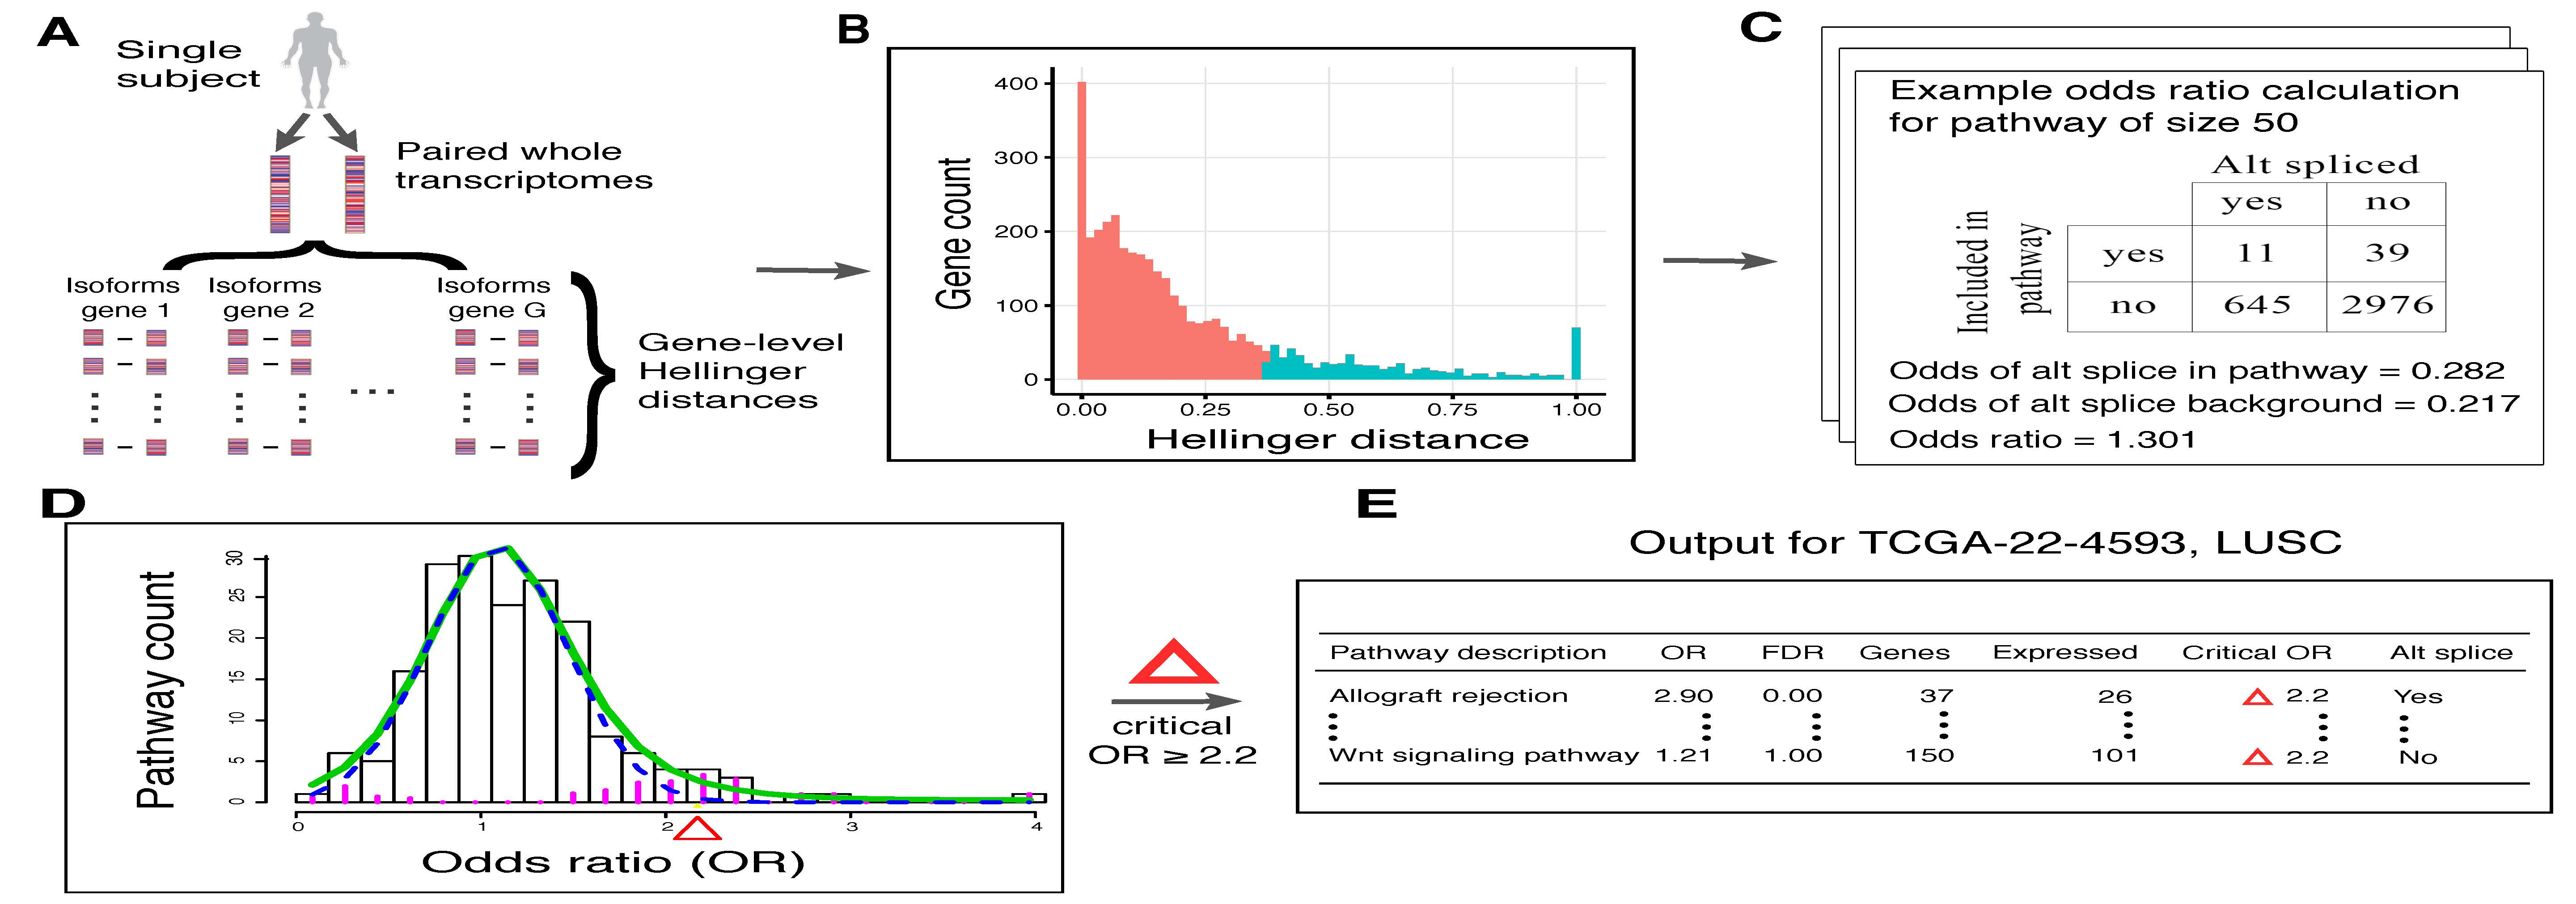
\includegraphics[width=\paperwidth]{figures/Figure1.jpg} }
  \begin{frame}[plain] 

     \vskip60pt
  \begin{TitleBox}
    {\huge \inserttitle} 
    \vskip5pt
    {\large\insertauthor}\\
    \insertinstitute\\
    %{\footnotesize \href{http://twitter.com/adaptive_plant}{{\FA \faTwitter} adaptive\_plant}
    %\href{http://www.falsters.net/daniel}{{\FA \faHome} www.falsters.net/daniel}
    %\href{mailto: daniel.falster@mq.edu.au}{{\FA \faEnvelope}  daniel.falster@mq.edu.au}
    % }
    \vskip3pt
%%    {\footnotesize Statistical advisor:~Dr.~Walter W.~Piegorsch}\\
%%        {\footnotesize Biomedical informatics advisor:~Dr.~Yves A.~Lussier}
    {\footnotesize
      \Email\href{mailto: aschissler@unr.edu}{aschissler@unr.edu}\\
      \Mundus\href{http://www.grantschissler.com}{www.grantschissler.com}
    }
   \end{TitleBox}

 \end{frame}

}

%% the title page
%% \begin{frame}[plain]
%% \titlepage
%% \end{frame}

%% Outline
%%\begin{frame}
%%  \frametitle{Presentation outline}
%%    \tableofcontents
%%  % \tableofcontents[pausesections]
%%  \note{As there is a lot to cover, let me step through an outline of this talk.}
%%  \note{First, quickly provide some motivating data and essential background.}
%%  \note{Then, we\rq ll discuss in detail the statistical method development and evaluation.}
%%  \note{Time allowing, present some key results, visualizations, and an R implementation.}
%%  \note{Lastly, I\rq ll quickly summarize the work and future directions.}
%%\end{frame} 
%%



%%%% Part I: Precision medicine motivation
%% \section{Aims \& big ideas}
%% \subsection{Aims \& big ideas}

 \section{Background \& Prior work}
\subsection{Aims \& motivating data}
 
\begin{frame}\frametitle{The general idea}
\begin{itemize}
\item We'd like a methodology to estimate complex biological dysregulation using paired samples from cancer patients.
\item This dysregulation relates to coordinated differential protein isoform usage within biological pathways.
\item But we seek a single-subject framework for precision medicine.
\item Moreover, the setting involves large-scale simultaneous signification under correlated test statistics.
  \item This is extremely challenging when you only can analyze one patient's data at a time!
\item I'll also discuss challenges in interdisciplinary statistics (e.g, fast initial model development, your method must ``work'' statistically but also reveal biological insights (validation!).
\end{itemize}
\end{frame}

\begin{frame}\frametitle{This work is an invited manuscript to Frontiers in Genetics}
\begin{figure}[htb]
  \centering 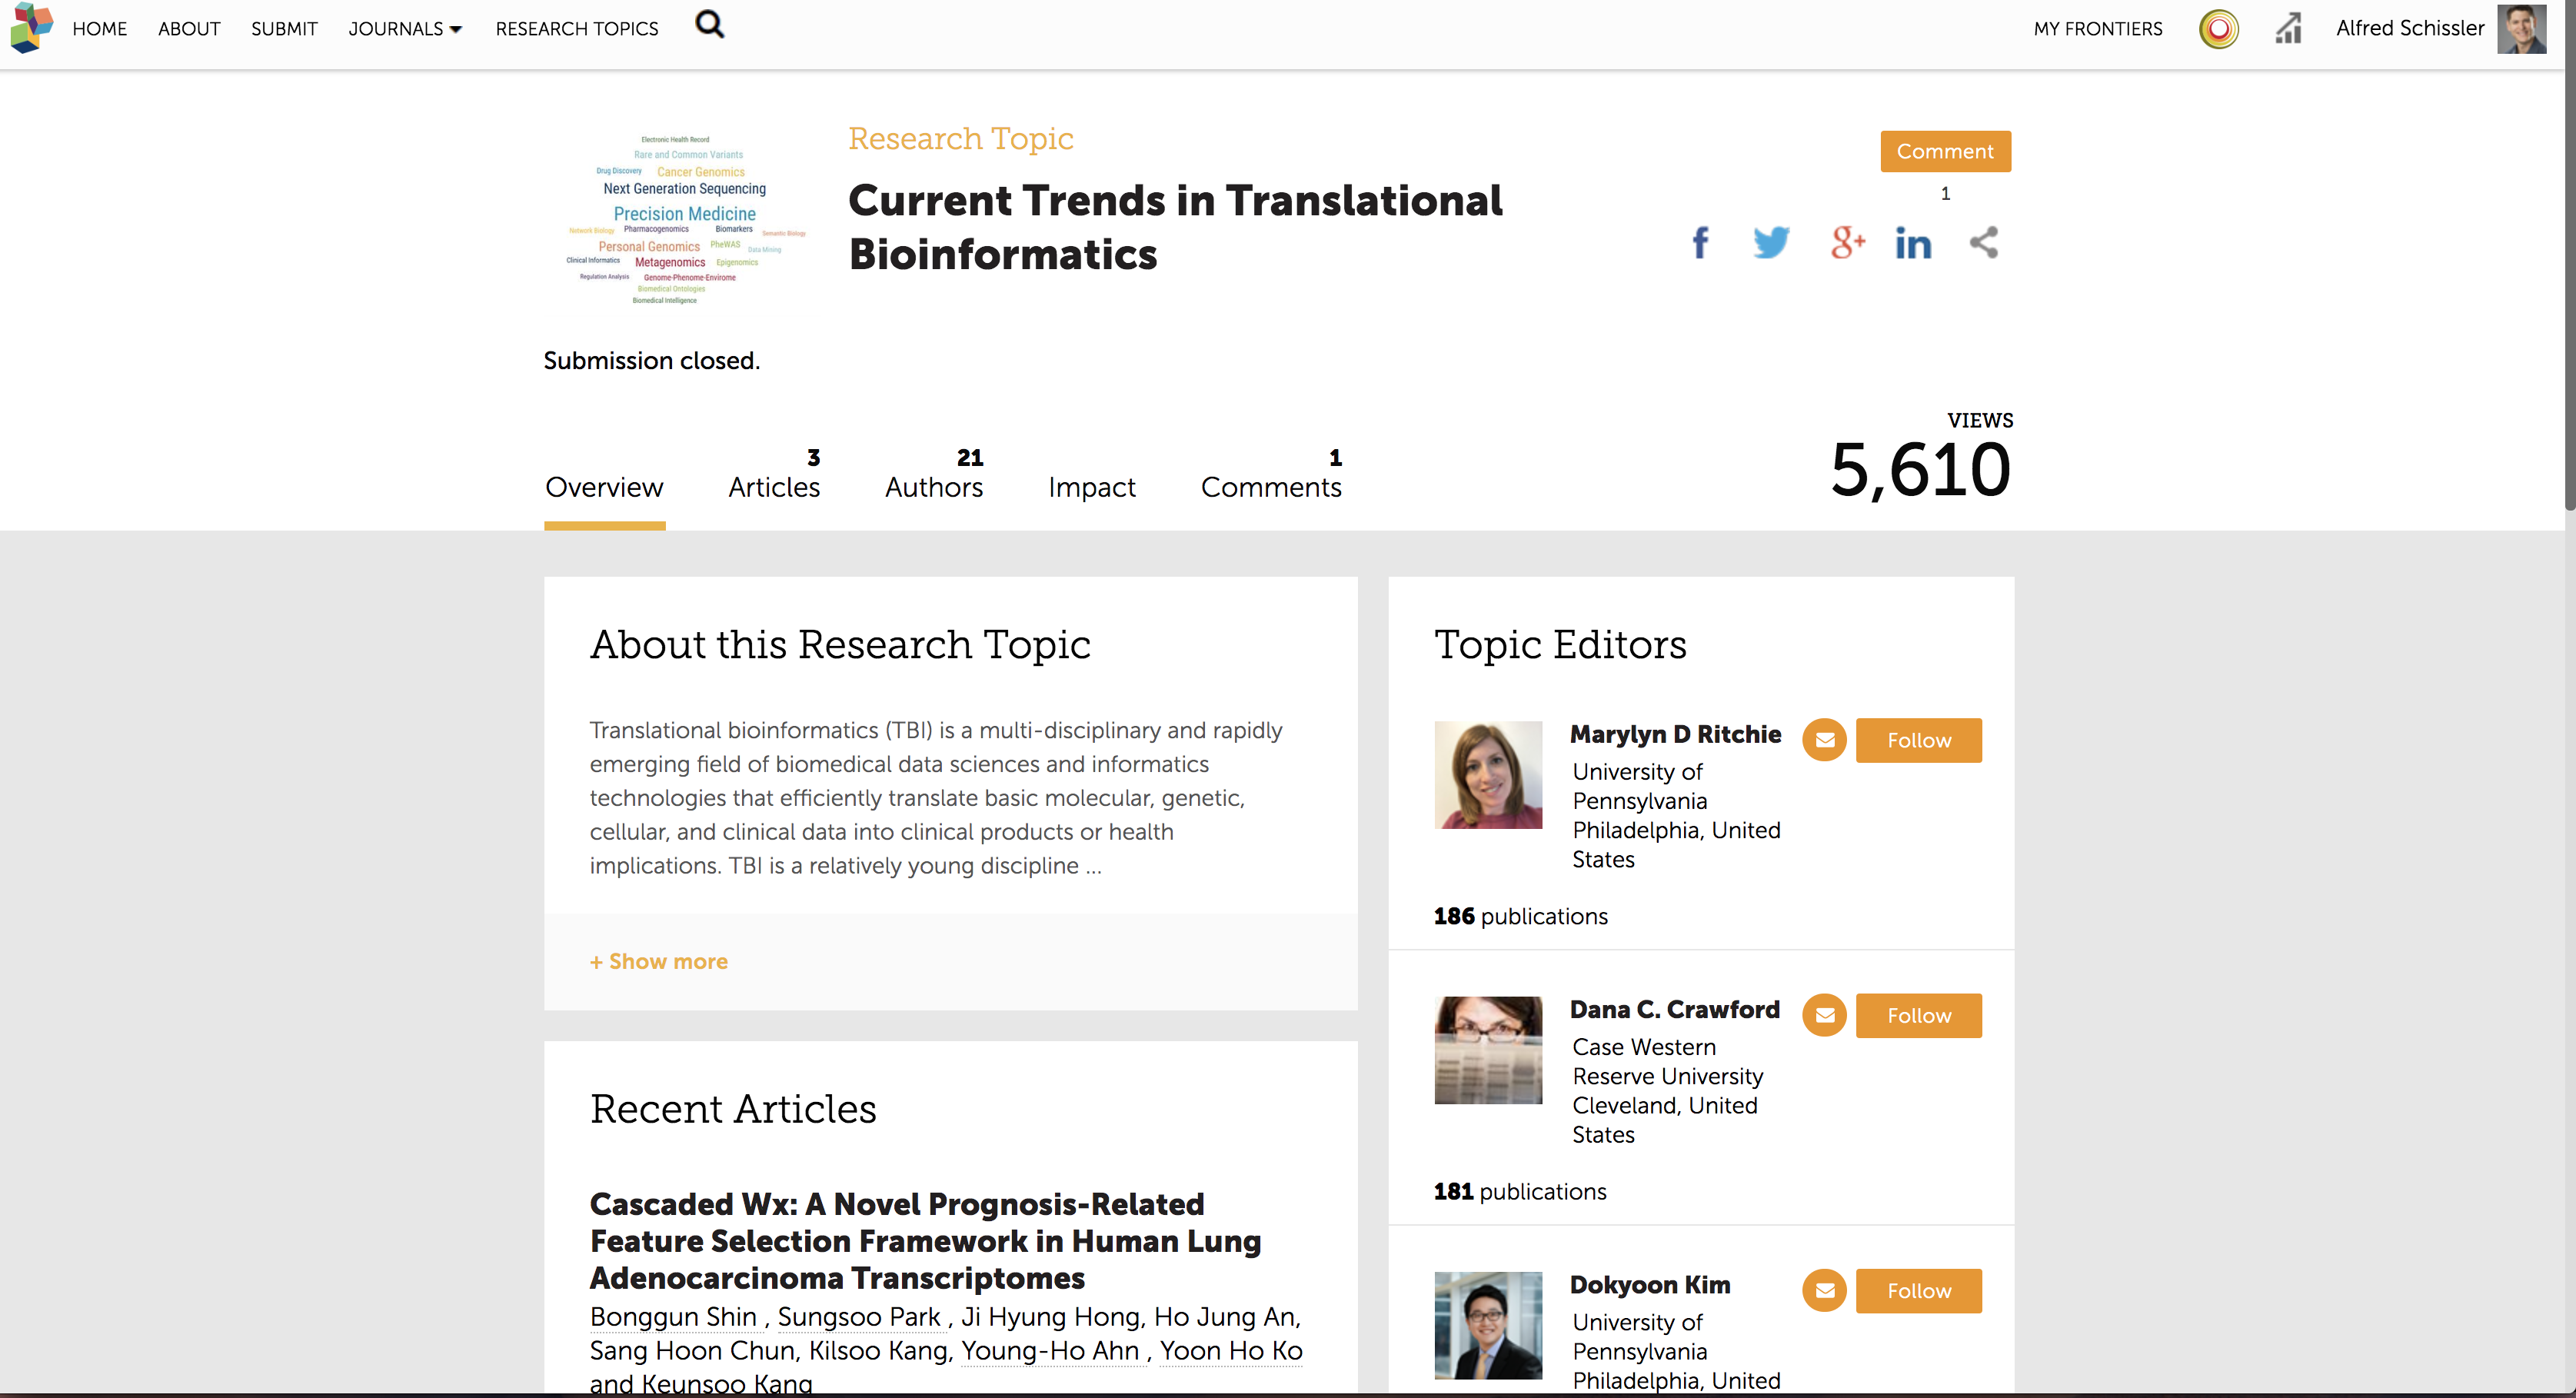
\includegraphics[keepaspectratio,width=\textwidth,height=0.8\textheight]{figures/frontiers10152019.png}
\end{figure}
\end{frame}

%% \subsection{Motivating data}
%\begin{frame}\frametitle{Example paired RNA-seq\addtocounter{footnote}{-2}\footnotemark ~quantified mRNA (normalized) expression data in a gene set\footnotemark}
  \begin{frame}\frametitle{RNA-seq isoform counts from lung cancer tumors\addtocounter{footnote}{-1}\footnotemark}
  \begin{table}
\label{tab:TNBCdata}
\begin{tabular}{c|l|ccc}
\hline
$i$ & Gene symbol & Isoform ID & Normal & Tumor \\
\hline
1 &  \emph{DDX11L1}   & uc011lsn.1  & 0   & 0 \\
2 &  \emph{DDX11L9}     & uc010unu.1  & 2   & 23 \\
3 &  \emph{DDX11L1}    & uc010uoa.1  & 0   & 0 \\
4 &  \emph{OR4F5}   & uc002bgz.2  & 8   & 16 \\
5 &  \emph{DQ597235}     & uc002bic.2  & 0   & 0 \\
6 &  \emph{DQ599768}    & uc010zzl.1  & 115 &   159 \\
$\vdots$ &   $\vdots$       & $\vdots$ & $\vdots$ & $\vdots$  \\
73599 &  \emph{abParts}  & uc011nby.1  & 0   & 0  \\
\hline
\end{tabular}
\end{table}
\addtocounter{footnote}{1}\footnotetext{The Cancer Genome Atlas (TGCA) LUSC data set}
% \addtocounter{footnote}{1}\footcitetext{TCGA}
% \addtocounter{footnote}{1}\footcitetext{Won2013g}

\end{frame}

 \begin{frame}\frametitle{Alternatively spliced genes (ASGs) in a few pictures\addtocounter{footnote}{-1}\footnotemark}
   \begin{figure}[htb]
   \centering
 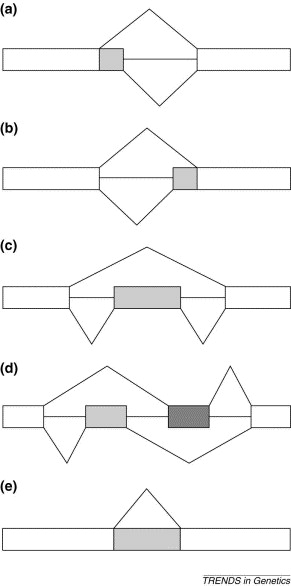
\includegraphics[keepaspectratio,width=\textwidth,height=0.75\textheight]{figures/splice_figure.jpg}
    \end{figure}
    \note{enormous diversity possible (some genes code for 10s of 1000s mRNAs}
    \addtocounter{footnote}{1}\footcitetext{Graveley2001}
  \end{frame}

%%  
%%\begin{frame}\frametitle{Why is studying individualized dysregulation important?}
%%  \begin{itemize}
%%  \item Cohort-derived cancer biomarkers are notoriously difficult to produce effective therapies for all patients\footcite{Kern2012}.
%%  \item This leads to the recent attention on developing precision medicine\footcite{Hamburg2010}.
%%  \item Some even speculate that N-of-1 is the ``ultimate strategy for individualizing medicine''\footcite{Lillie2011}.
%%  \item Moreover, small studies are cost efficient and allow investigation into rare disease.
%%  \end{itemize}
%%\end{frame}

 \subsection{Gene set analysis}
 \begin{frame}\frametitle{Gene set analysis in biomedical research}
   Gene set analyses\footcite{Khatri2012n1pas} give mechanistic interpretation by aggregating gene-level results. Widely-used method:~GSEA \footcite{Subramanian2005}. Example ontology:~KEGG\footcite{kanehisa2000kegg}.\\
   % \pause
     \begin{block}{Kyoto encyclopedia of genes and genomes (KEGG)}
       \begin{center}
         \begin{tabular}{lll}
           ID & Description & Gene\\
           \hline
           hsa00010 & Glycolysis Gluconeogenesis & LDHAL6B\\
           hsa00010 & Glycolysis Gluconeogenesis & ADH1B\\
           $\vdots$ & $\vdots$ & $\vdots$\\
           hsa05416 & Viral myocarditis & MYH8\\
         \end{tabular}
       \end{center}
     \end{block}
\end{frame}

\subsection{The N-of-1-{\itshape pathways} framework}
\begin{frame}\frametitle{The N-of-1-{\itshape pathways} framework\addtocounter{footnote}{-1}\footnotemark}
  \begin{figure}[htb]
    \centering
\includegraphics[keepaspectratio,width=\textwidth,height=0.6\textheight]{figures/N-of-1-pathways-dep-flowchart.pdf}
\end{figure}
%\pause
   \addtocounter{footnote}{1}\footcitetext{Gardeux2014}
\note{Smart dimension reduction of the transcriptome}
\note{Move quickly on this slide.}
\note{Mention the shortcomings}
\end{frame}

\subsection{Correlation and Large-Scale Simultaneous Significance Testing}
\begin{frame}\frametitle{Correlation and Large-Scale Simultaneous Sign.~Testing\addtocounter{footnote}{-1}\footnotemark} 
  \begin{figure}[htb]
  \centering
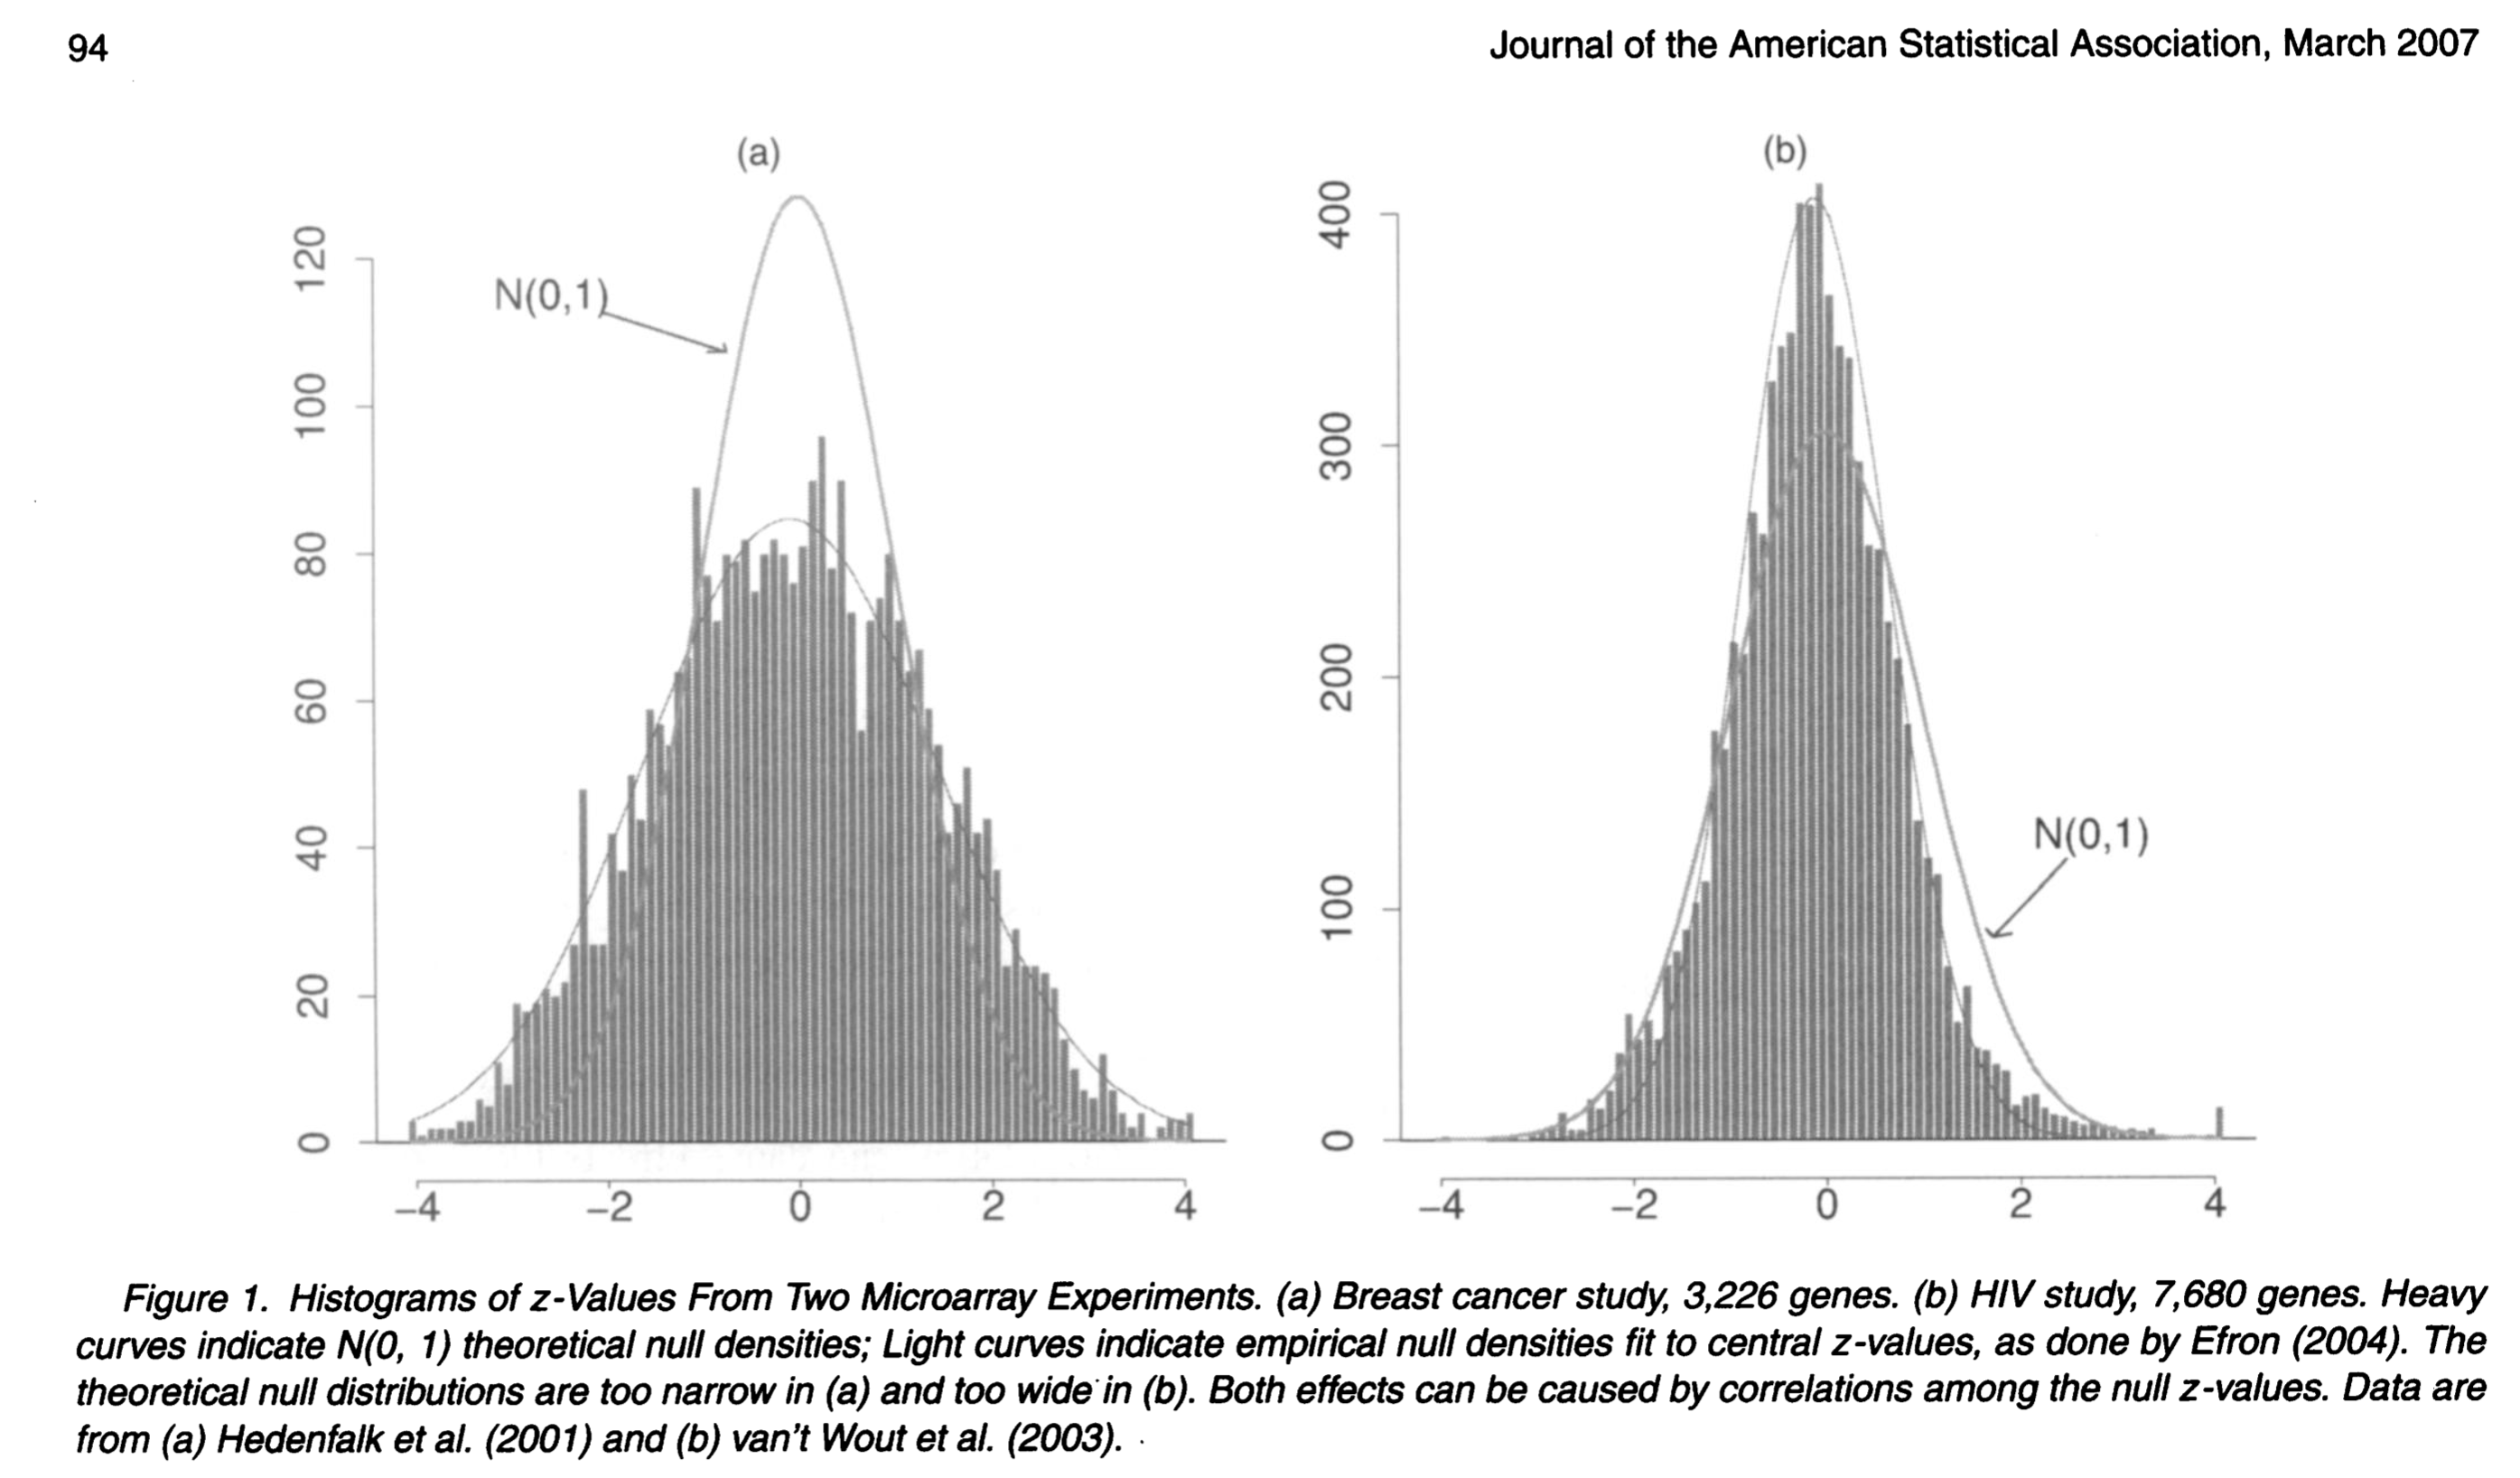
\includegraphics[keepaspectratio,width=\textwidth,height=0.75\textheight]{figures/Efron2007_figure1.png}
   \end{figure}
   \addtocounter{footnote}{1}\footcitetext{Efron2007a}
 \end{frame}

 \begin{frame}\frametitle{Efron's local false discovery rate\addtocounter{footnote}{-1}\footnotemark}
   Assume that $N$ values can be sorted into two classes ('null' and 'nonnull'), occurring with probabilities of $p_{0}$ or $p_{1}=1-p_{0}$,
   \begin{align*}
     p_{0} & = Pr\{null\} & f_{0}(z), if \; null \\
     p_{1} & = Pr\{nonnull\} & f_{1}(z), if \; nonnull
   \end{align*}
   Define the \emph{null subdensity} as $f^{+}_{0}=p_{0}f_{0}(z)$ and the \emph{mixture density} as $f(z)=p_{0}f_{0}(z) + p_{1}f_{1}(z)$. Then define the local false discovery rate (locFDR) as the Bayesian posterior probability that a case is null given $z$,

   \begin{equation*}
fdr(z) = Pr\{null | z \} = \frac{p_{0}f_{0}(z)}{f(z)}= f^{+}_{0}/f(z).
     \end{equation*}
   \addtocounter{footnote}{1}\footcitetext{Efron2013}
 \end{frame}

\subsection{Quantification of differential alternative splicing}
\begin{frame}\frametitle{Hellinger distance} 
  We follow Johnson \& Purdom\addtocounter{footnote}{-1}\footnotemark and use of the Hellinger distance to quantify alternative splicing between a pair of samples. Let the estimates of isoform expression for a sample $A$ be denoted as $x_{gA1},\ldots,x_{gAK_{g}}$ for the $K_{g}$ distinct isoforms annotated to gene $g$. We define the relative isoform usage as the vector of relative proportions of each isoform,
  $p_{gA}= \left( \frac{x_{gA1}}{\sum_{k=1}^{K_{g}} x_{gAk}}, \ldots, \frac{x_{gAK_{g}}}{\sum_{k=1}^{K_{g}} x_{gAk}} \right)$

  Then define the Hellinger distance
  \begin{equation*}
H_{g}(p_{gA}, p_{gB}) = 1 / \sqrt{2} \sum_{k=1}^{K_{g}} \left( \sqrt{ \frac{x_{gAk}}{\sum_{k=1}^{K_{g}} x_{gAk}}  }  - \sqrt{ \frac{x_{gBk}}{\sum_{k=1}^{K_{g}} x_{gBk}} } \right)^{2}
    \end{equation*}
 \addtocounter{footnote}{1}\footcitetext{Johnson2017}
 \end{frame}

\section{Method development}
 
\subsection{N-of-1-pathways Alternatively Spliced (N1PAS)}

\begin{frame}\frametitle{N-of-1-pathways Alternatively Spliced (N1PAS)}
\begin{figure}[htb]
  \centering 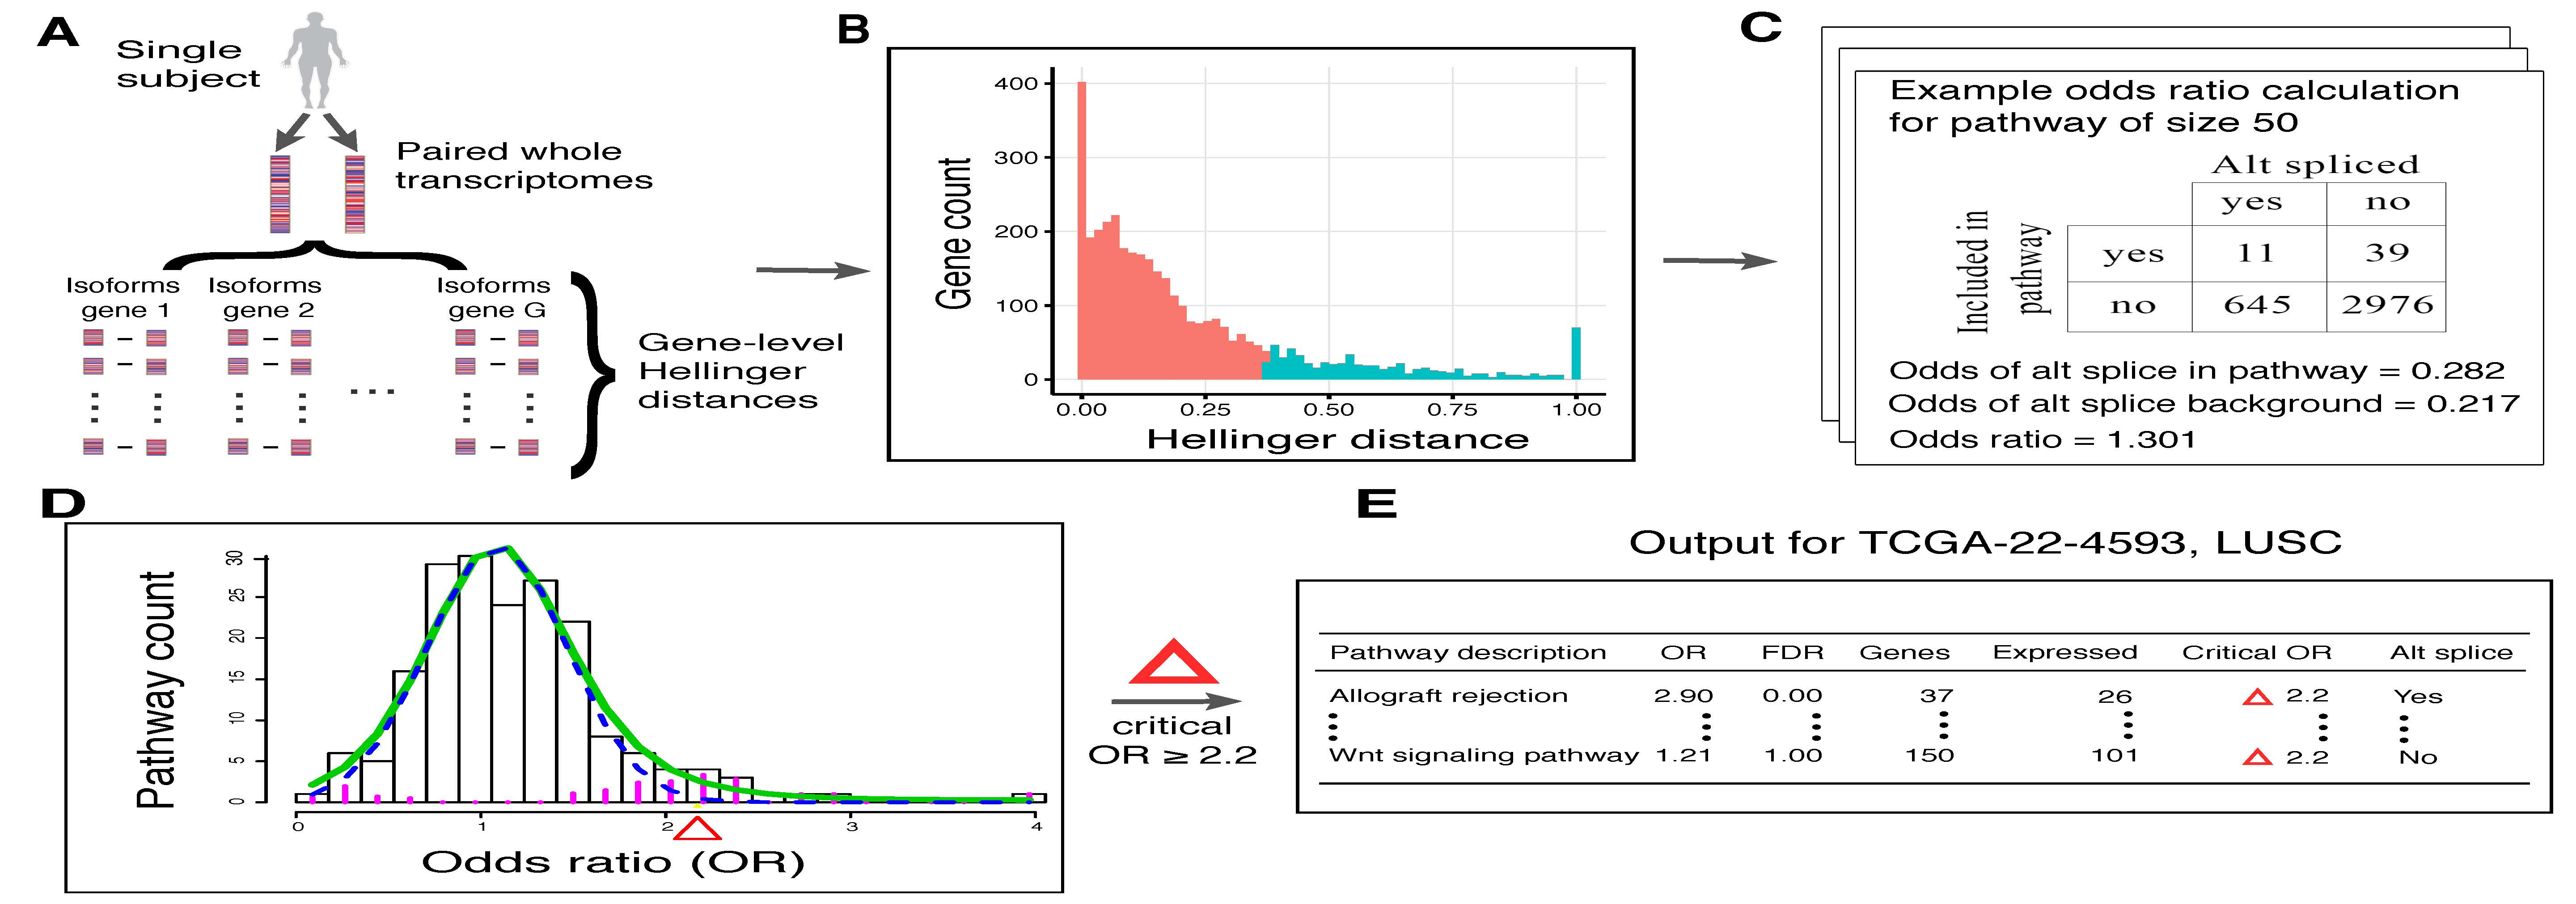
\includegraphics[keepaspectratio,width=\textwidth,height=0.8\textheight]{figures/Figure1.jpg}
\end{figure}
\end{frame}

\begin{frame}\frametitle{TCGA data sets to guide development}
\begin{figure}[htb]
  \centering 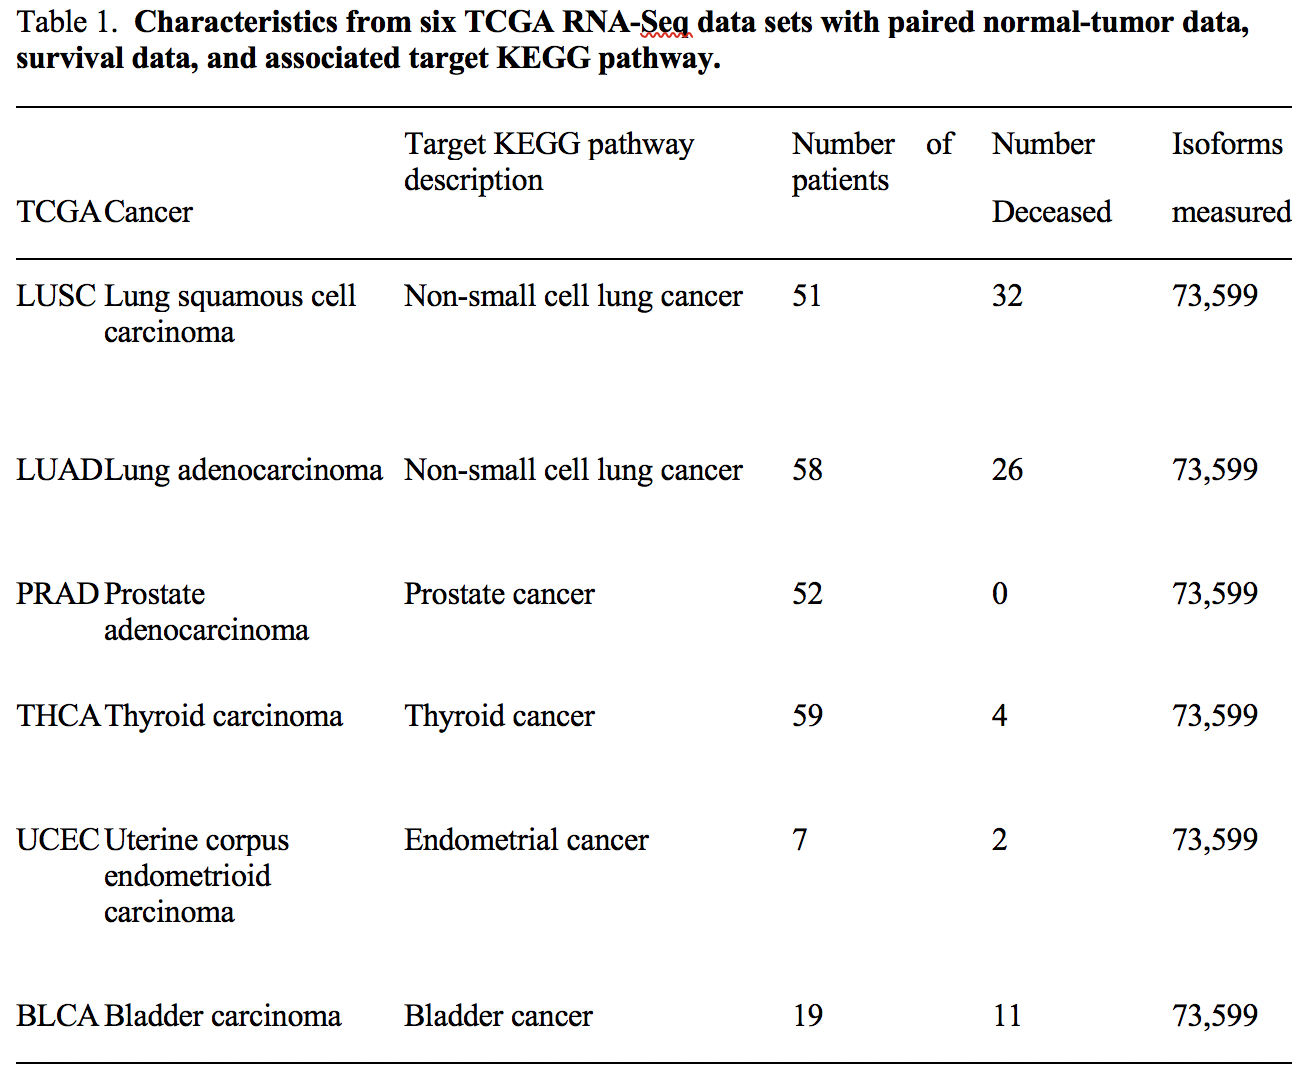
\includegraphics[keepaspectratio,width=\textwidth,height=0.8\textheight]{figures/datasets.png}
\end{figure}
\end{frame}

\subsection{Monte Carlo evaluation}

\begin{frame}
  \frametitle{Monte Carlo study design and challenges}
  \begin{itemize}
  \item Trying the simulate parameterically is challenging as the isoform counts are ultra high-dimensional, multivariate, and discrete
  \item Instead we chose to permute in a subject-specific way:~find the distribution of Hellinger distances for the 4133 genes annotated to KEGG pathways. Then permute gene labels to create null distribution of pathway odds ratios.
    \item The effect size corresponds to the proportion of ASGs within a pathway $\pi$, relative to the subject-specific background level of ASGs ($\pi_{all}$).
  \end{itemize}
\end{frame}

\begin{frame}\frametitle{Simulation settings and procedure}
  \begin{itemize}
    % \item 4 methods tested:\\(1) gpu-norta, (2) C-norta, (3) R-norta, (4) copula.
  \item 6 TCGA data sets explored, for a total of 246 patients.
    \item For each patient, compute Hellinger distances for each gene and use 2-means to cluster into ASG or not classes.
    \item Let $G=\{15, 30, 50, 100\}$ be the number of expressed genes in the specified pathway. Select at random a KEGG pathway with this number of genes.
    \item Let the effect size $\pi=\{0, 0.05, 0.10, 0.15, 0.20\}$.
    \item Select $G \times (\pi + \pi_{all})$ genes within the specified pathway at random to be from the ASG class and the remaining pathway genes from the non-ASG class.
    \item Apply N1PAS 100 times and determine empirical power as detection rate of the specified pathway.
      \item This results in 246 * 5 effect sizes * 4 pathway size * 100 reps = 492,000 simulated N1PAS runs.
\end{itemize}
\end{frame}

\begin{frame}\frametitle{Permutation-based simulated false discovery rates ($\pi=0$)}
  \begin{figure}[htb]
  \centering \includegraphics[keepaspectratio,width=\textwidth,height=0.8\textheight]{figures/Figure6noGeneSetSize_gs.pdf}
\end{figure}
\end{frame}

\begin{frame}\frametitle{Permutation-based simulated power}
  \begin{figure}[htb]
  \centering \includegraphics[keepaspectratio,width=\textwidth,height=0.9\textheight]{figures/Figure7.pdf}
\end{figure}
\end{frame}

\begin{frame}\frametitle{Permutation-based simulated power}
  \begin{figure}[htb]
  \centering 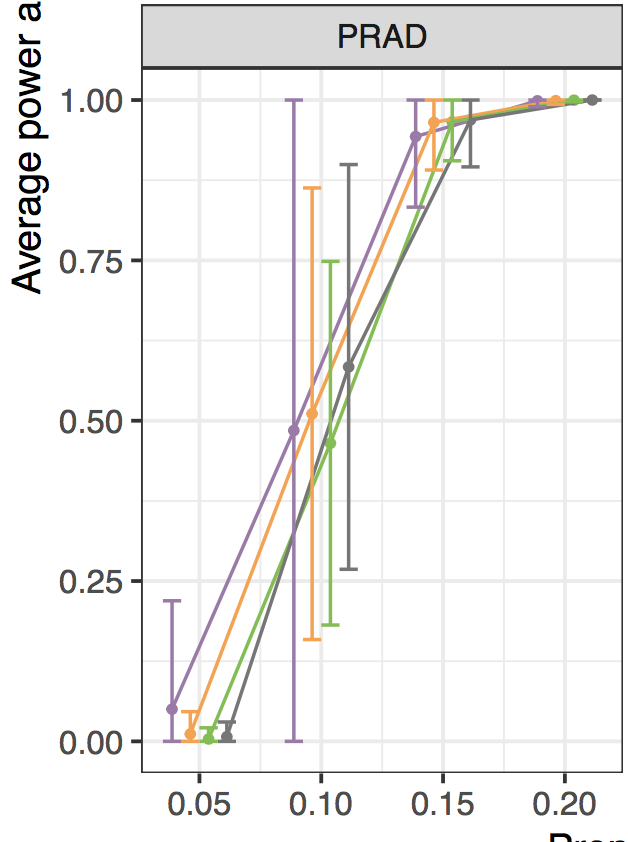
\includegraphics[keepaspectratio,width=\textwidth,height=0.9\textheight]{figures/Figure7_one.png}
\end{figure}
\end{frame}

\section{Method validation \& applications}
\subsection{KEGG target pathway study}
  
\begin{frame}
  \frametitle{Validation design and challenges}
  \begin{itemize}
  \item Validation is a major challenge in computational biology.
  \item Usually, in statistics, we just have to apply a proposed method to a data set and discuss results.
  \item Here, we have to both develop the method and show why we should care (i.e. find interesting or sensible results).
    \item So we designed a study to explore how often a \emph{target pathway} (pathway annotated the data set's cancer) was detected
  \end{itemize}
  
\end{frame}

\begin{frame}\frametitle{KEGG validation study results}
\begin{figure}[htb]
  \centering 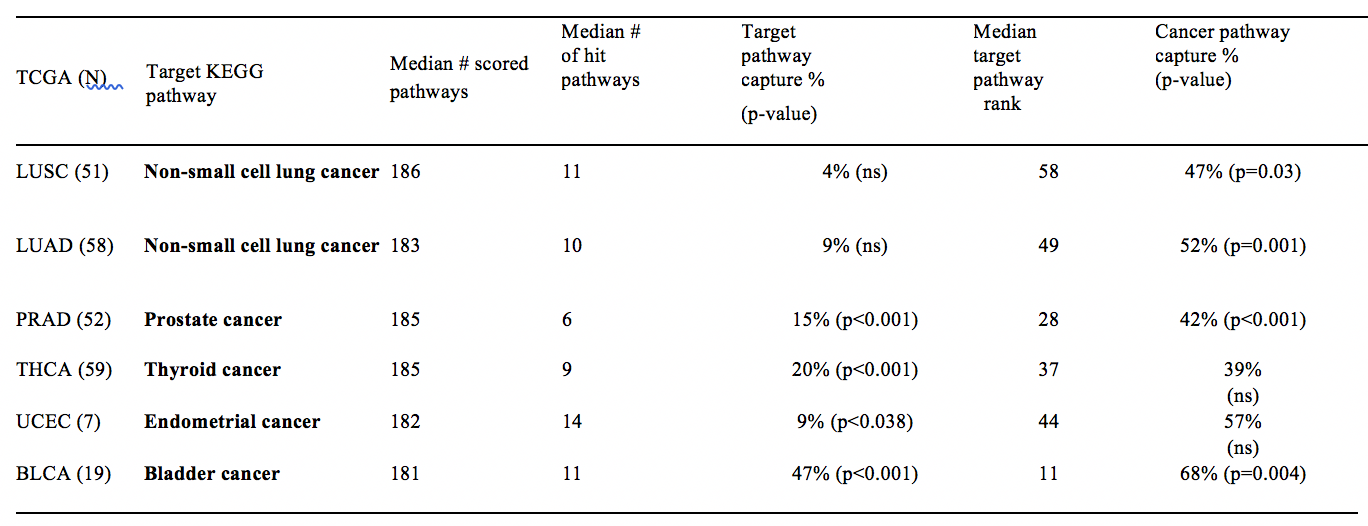
\includegraphics[keepaspectratio,width=\textwidth,height=0.8\textheight]{figures/table2.png}
\end{figure}
\end{frame}

\begin{frame}\frametitle{Boxplots of patient-specific odds ratios (OR) of the target KEGG pathway for the six TCGA data sets}
  \begin{figure}[htb]
  \centering 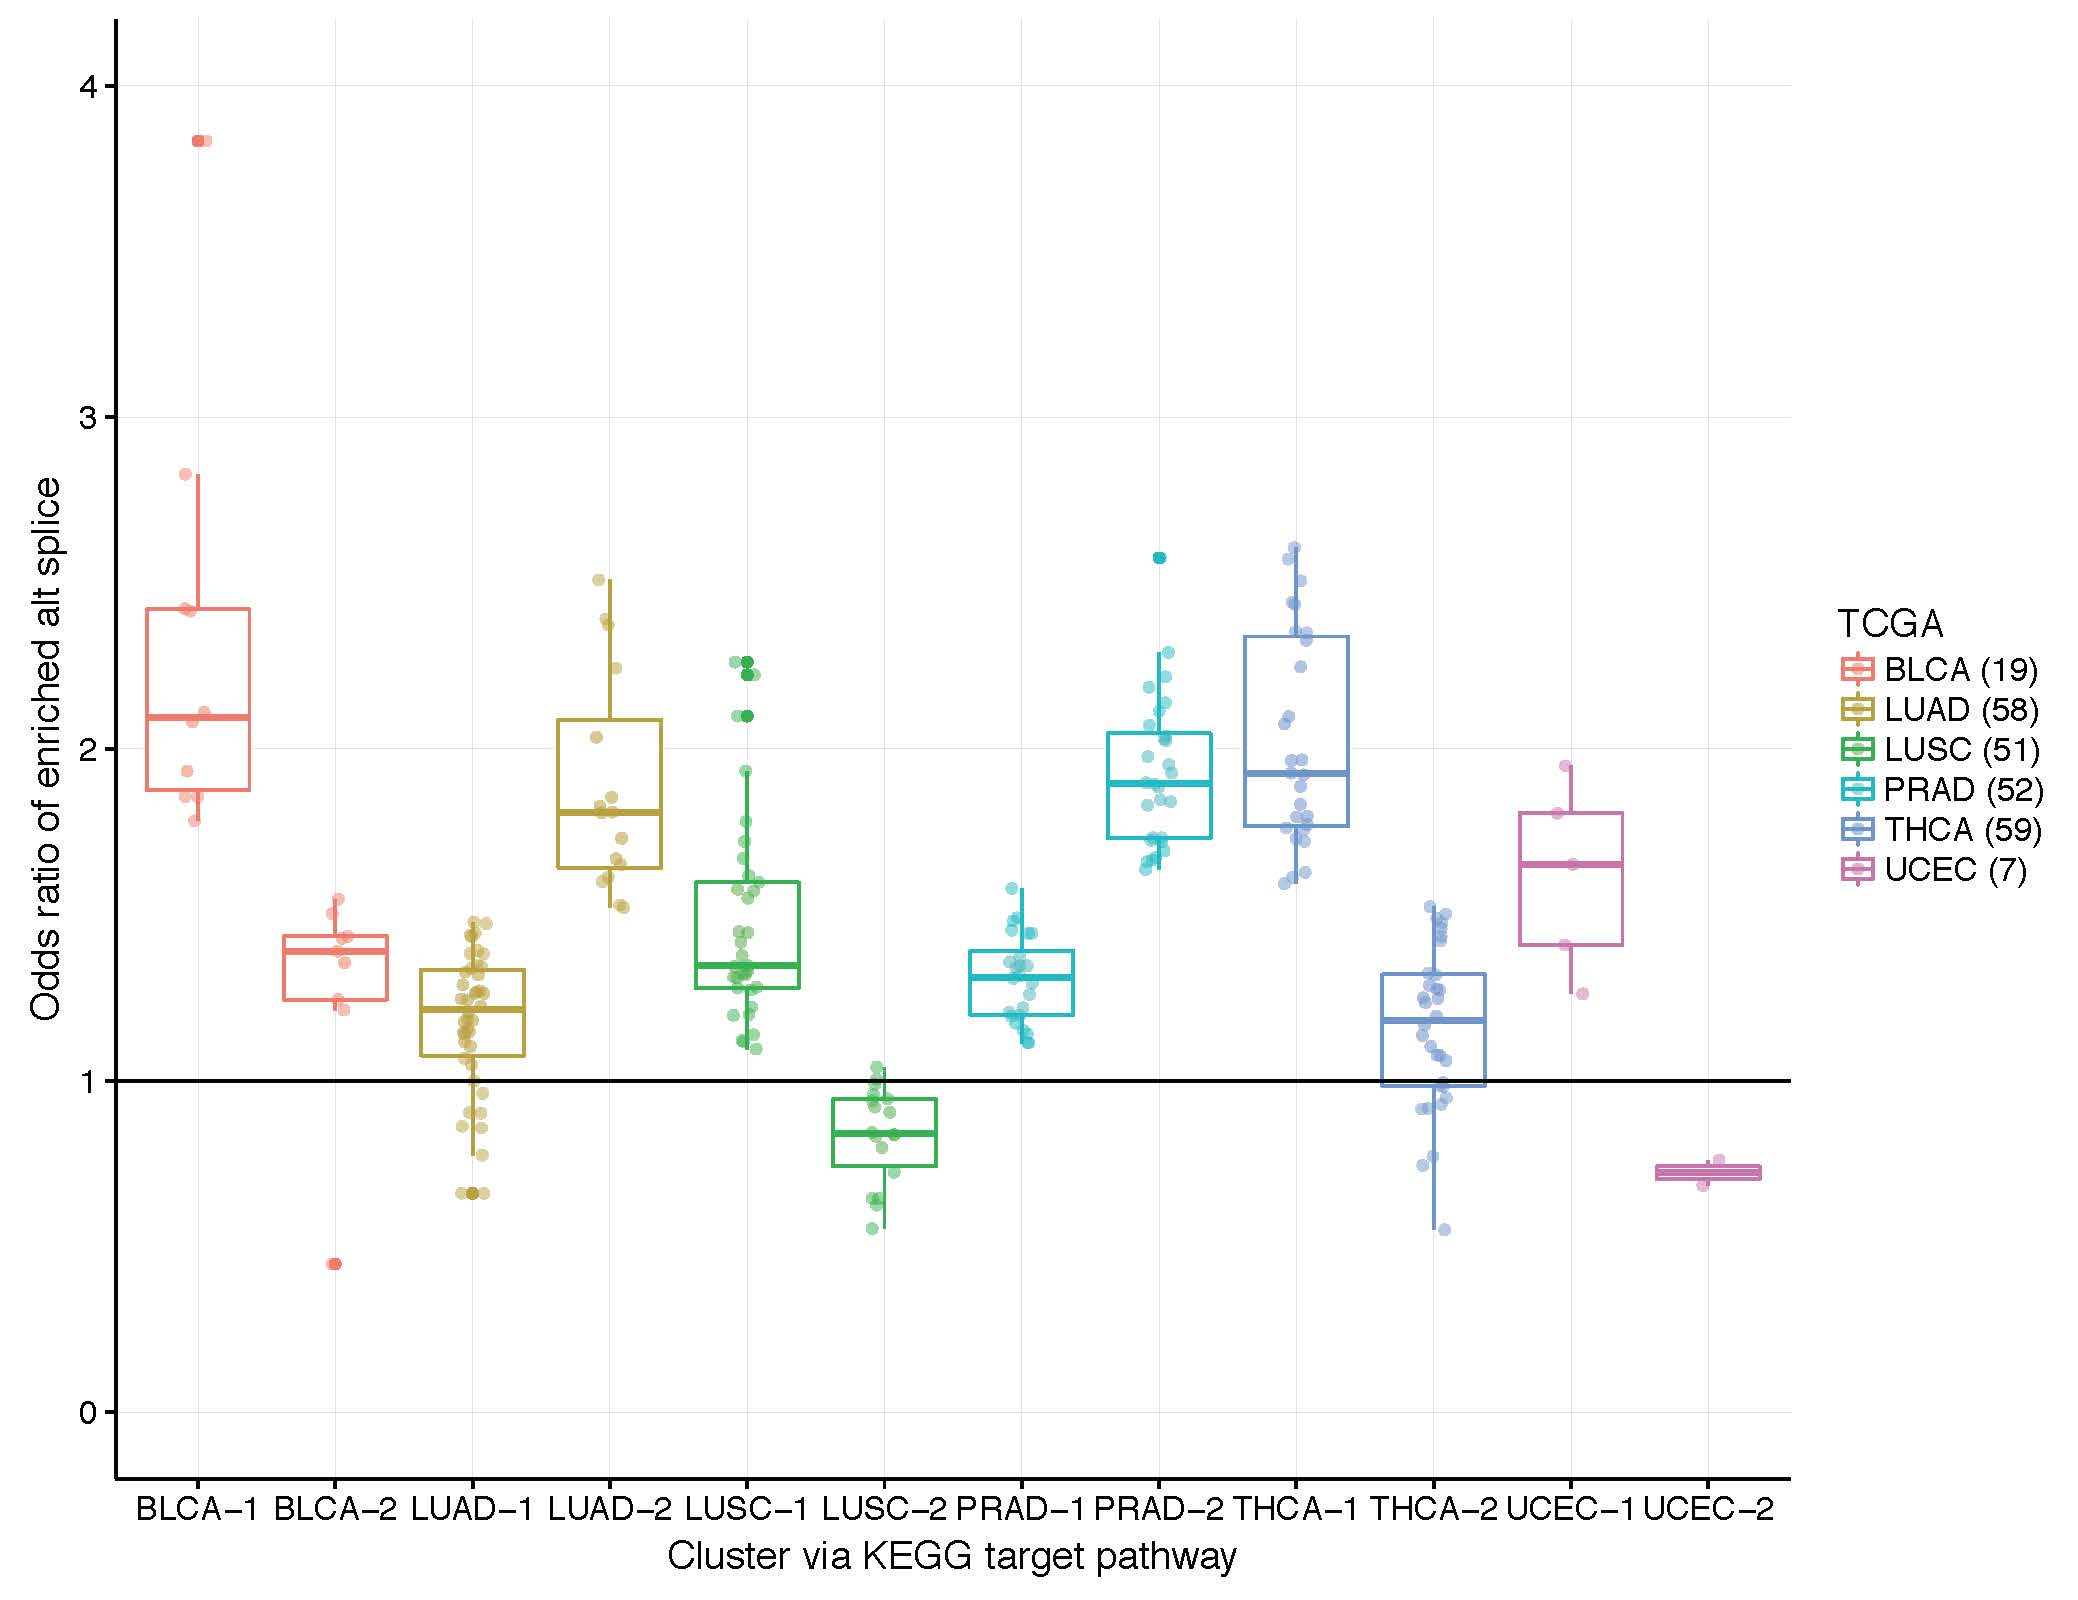
\includegraphics[keepaspectratio,width=\textwidth,height=0.8\textheight]{figures/Figure3.jpg}
\end{figure}
\end{frame}

\subsection{Survival subtyping pipeline \& alternative method comparison}

\begin{frame}\frametitle{Survival subtyping pipeline using N1PAS}
\begin{figure}[htb]
  \centering 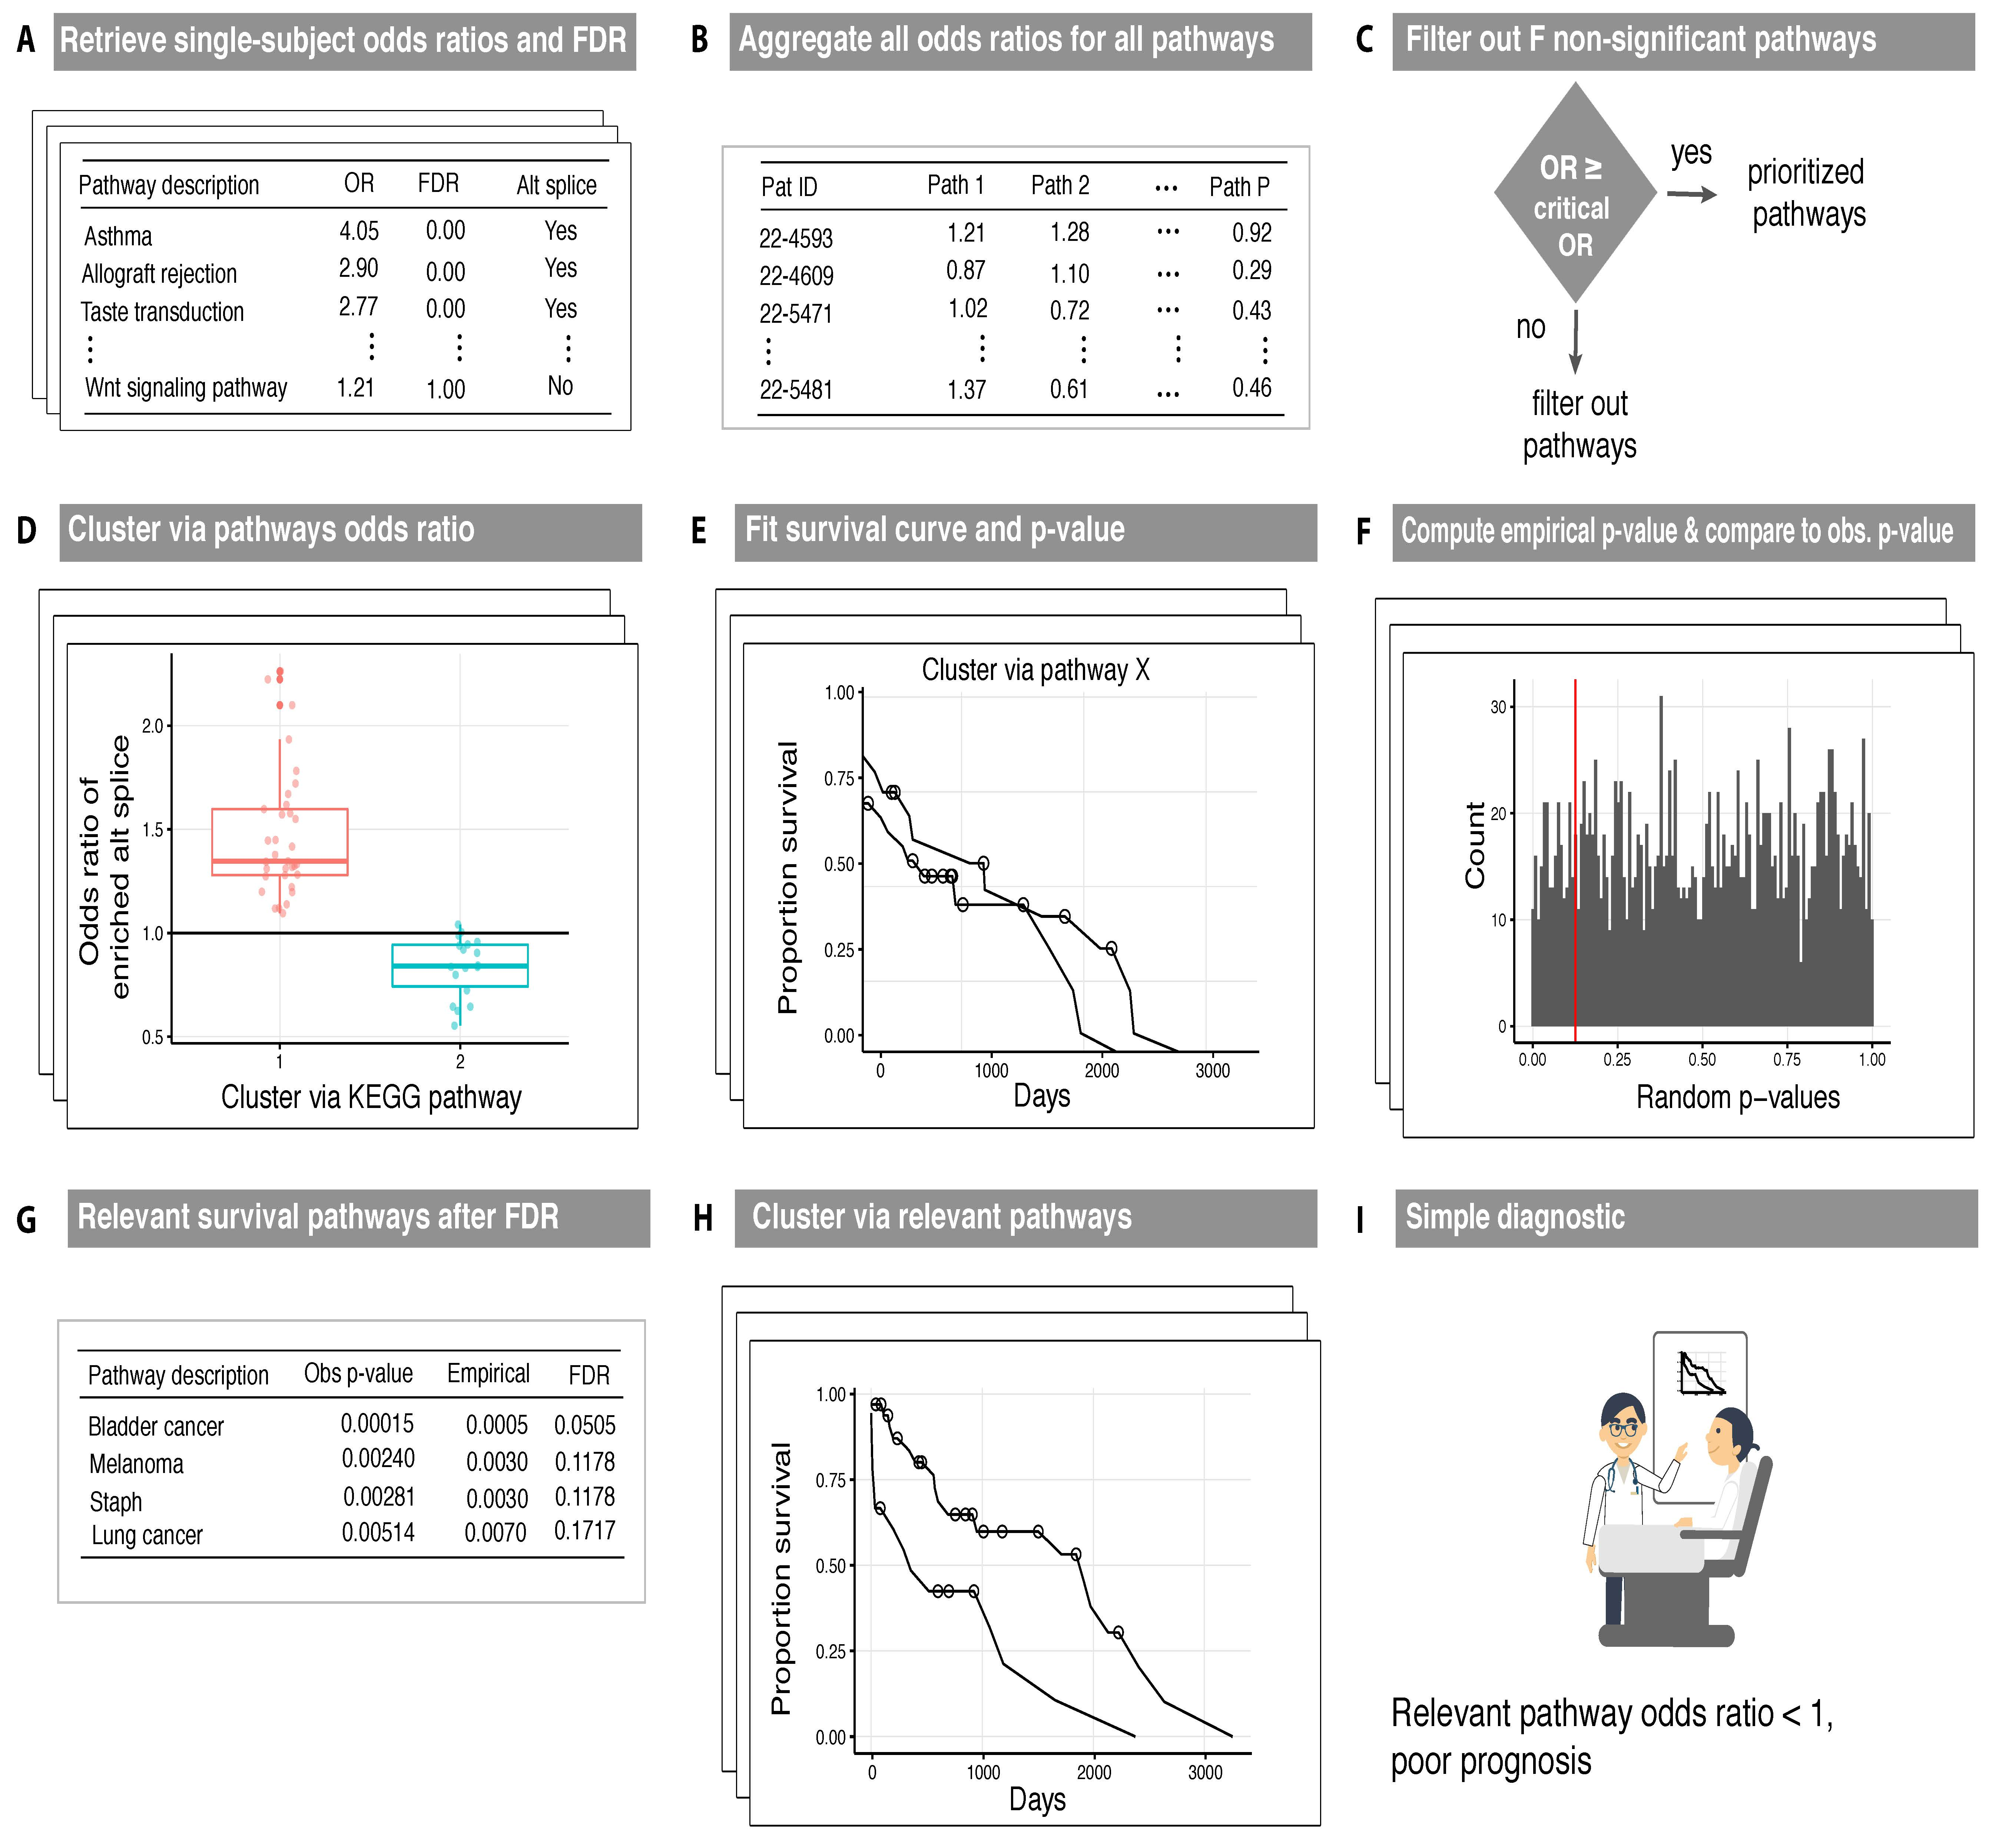
\includegraphics[keepaspectratio,width=\textwidth,height=0.8\textheight]{figures/Figure2.jpg}
\end{figure}
\end{frame}

\begin{frame}\frametitle{Non-small cell lung cancer (LUSC) pathways selected by subtyping pipeline}
\begin{figure}[htb]
  \centering 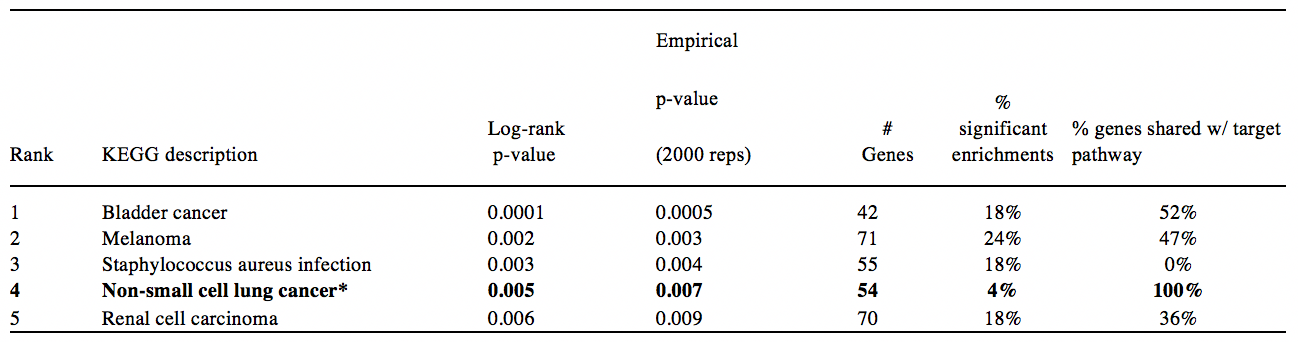
\includegraphics[keepaspectratio,width=\textwidth,height=0.8\textheight]{figures/table3.png}
\end{figure}
\end{frame}

\begin{frame}\frametitle{Clustering agreement Jaccard index}
  To quantify the agreement, we compute the Jaccard index as $J_{12}=\frac{|G_{1} \cap G_{2}|}{|G_{1} \cup G_{2}|}$, where $G_1,G_2$ are the sets of patients clustered using the 1st and 2nd top pathways (for either the Better or Worse subtype)
\begin{figure}[htb]
  \centering 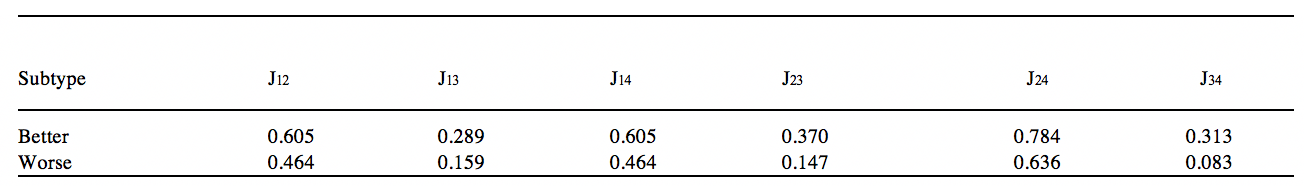
\includegraphics[keepaspectratio,width=\textwidth,height=0.8\textheight]{figures/table4.png}
\end{figure}
\end{frame}

\begin{frame}\frametitle{LUSC patient (N = 51, 32 deaths) survival curves}
  \begin{figure}[htb]
  \centering 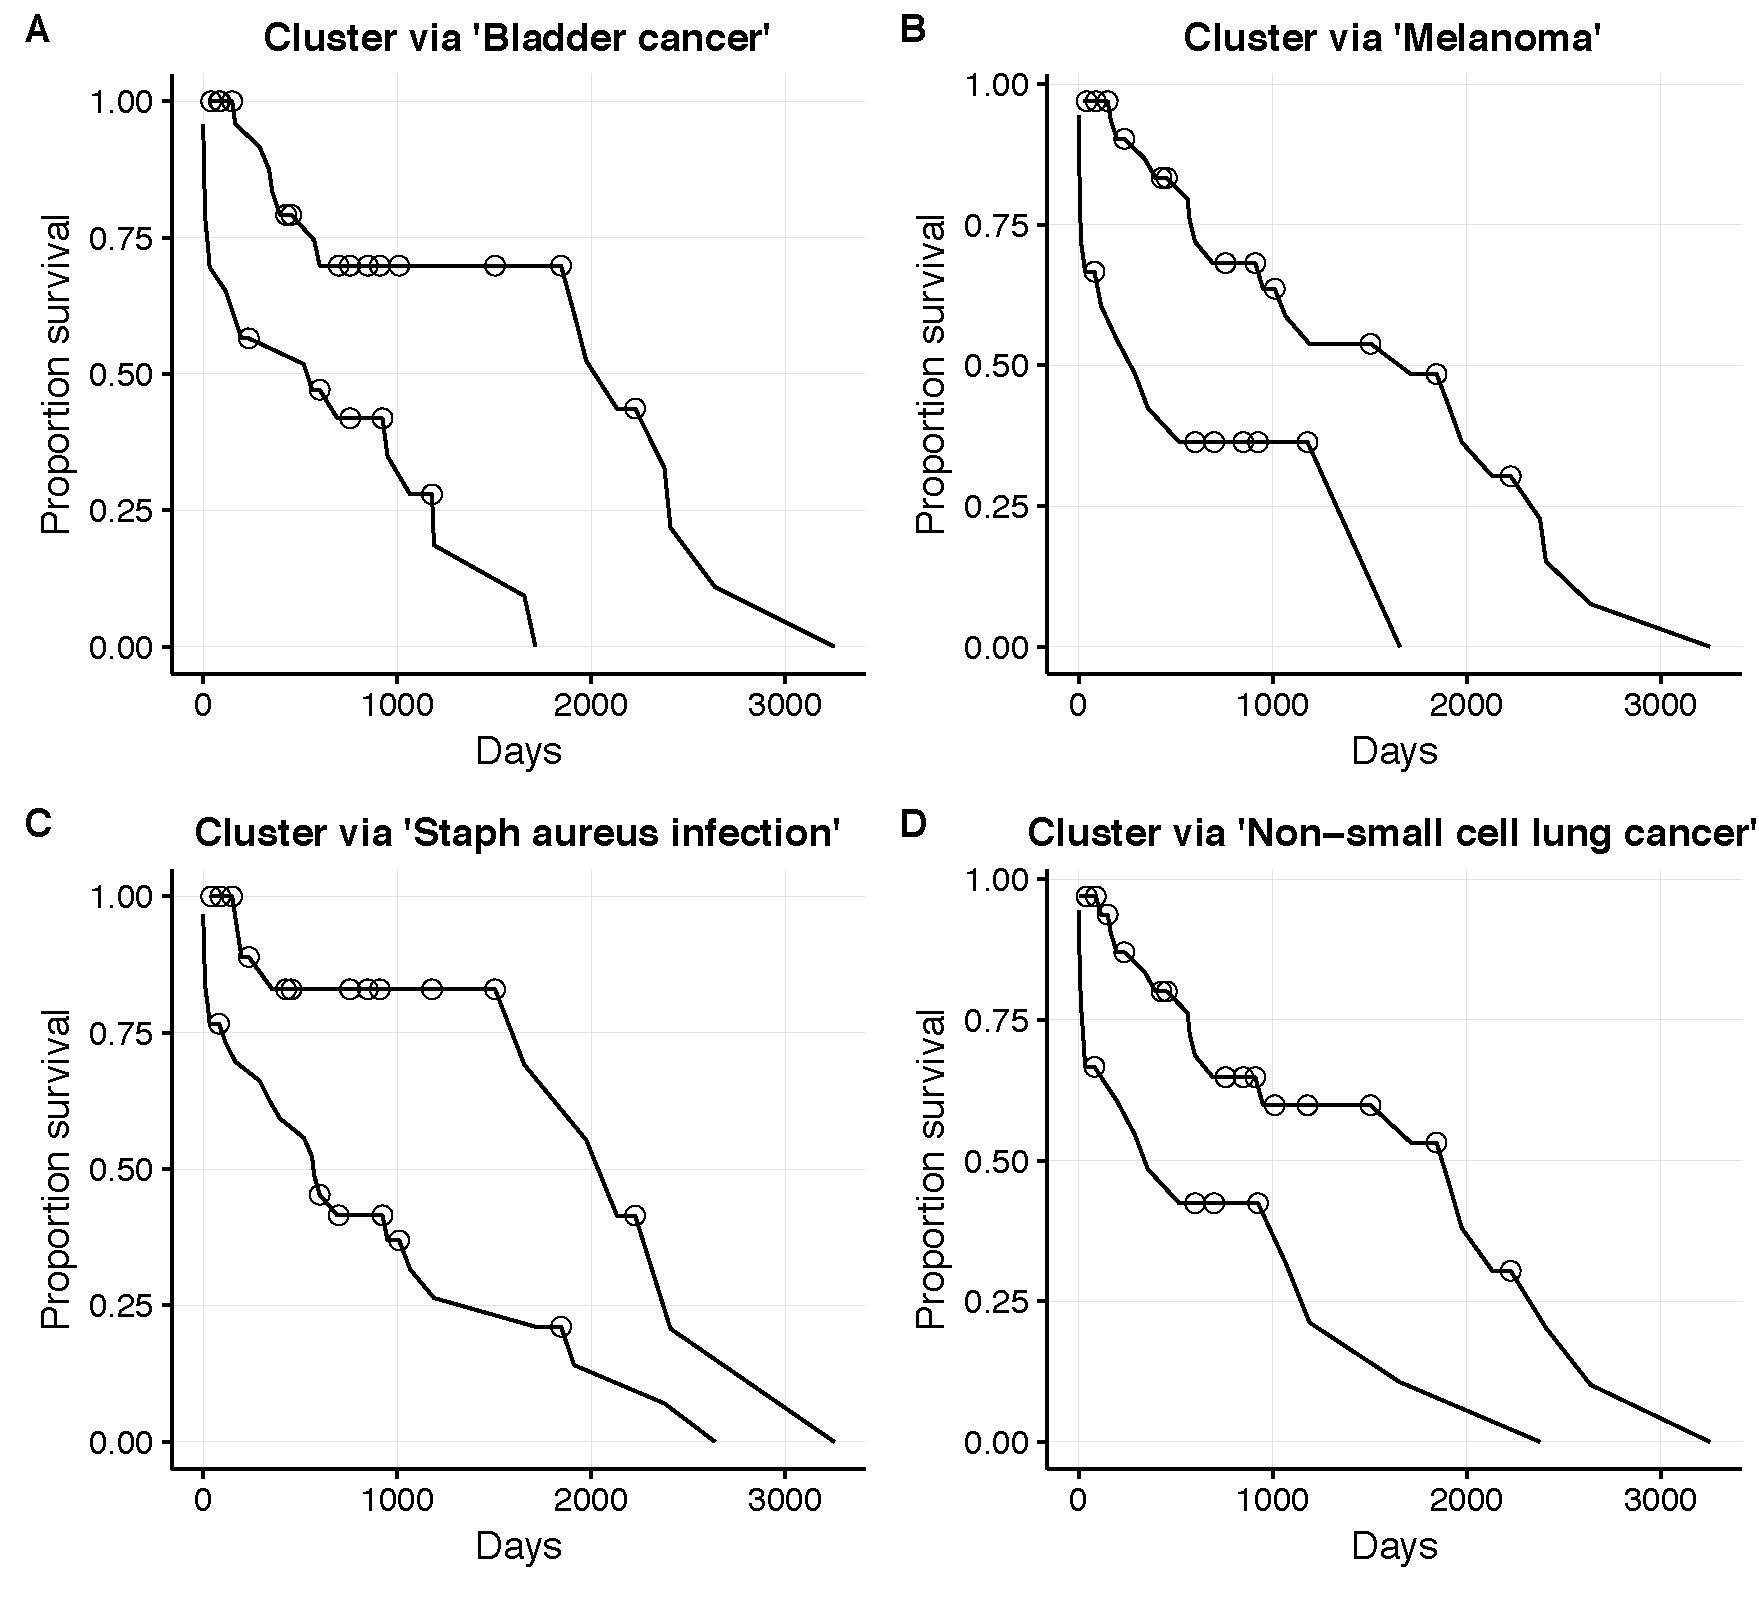
\includegraphics[keepaspectratio,width=\textwidth,height=0.8\textheight]{figures/Figure4.jpg}
\end{figure}
\end{frame}

\begin{frame}\frametitle{Boxplots overlaid with points indicating the odds ratios of pathway enriched with ASGs.}
  \begin{figure}[htb]
  \centering \includegraphics[keepaspectratio,width=\textwidth,height=0.8\textheight]{figures/Figure5_v5.pdf}
\end{figure}
\end{frame}

\begin{frame}\frametitle{Study of subtype clustering inputs using tumor isoform expression}
\begin{figure}[htb]
  \centering 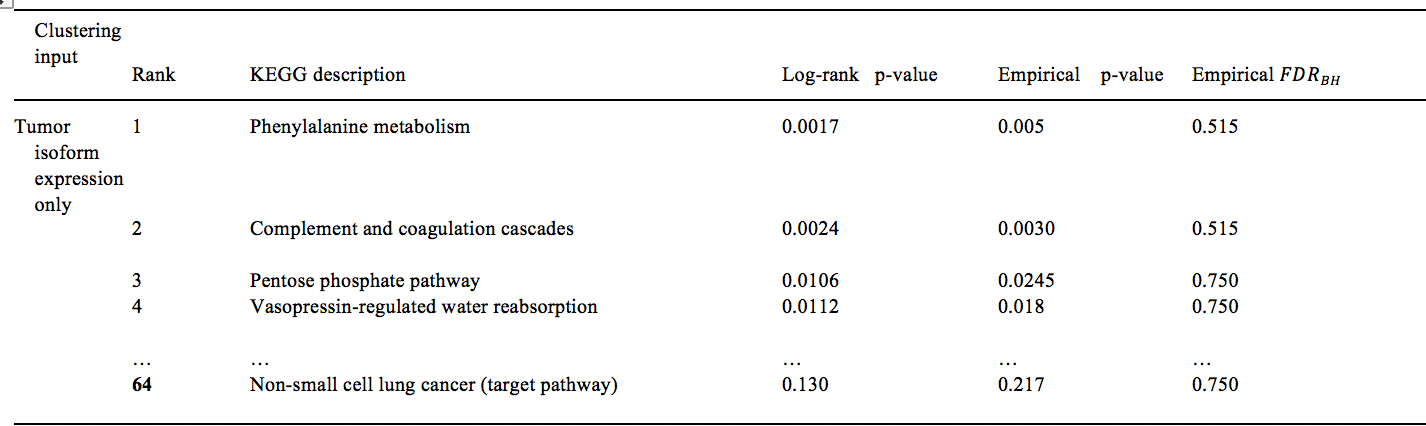
\includegraphics[keepaspectratio,width=\textwidth,height=0.8\textheight]{figures/table51.png}
\end{figure}
\end{frame}

\begin{frame}\frametitle{Study of subtype clustering inputs using difference in isoform expression}
\begin{figure}[htb]
  \centering 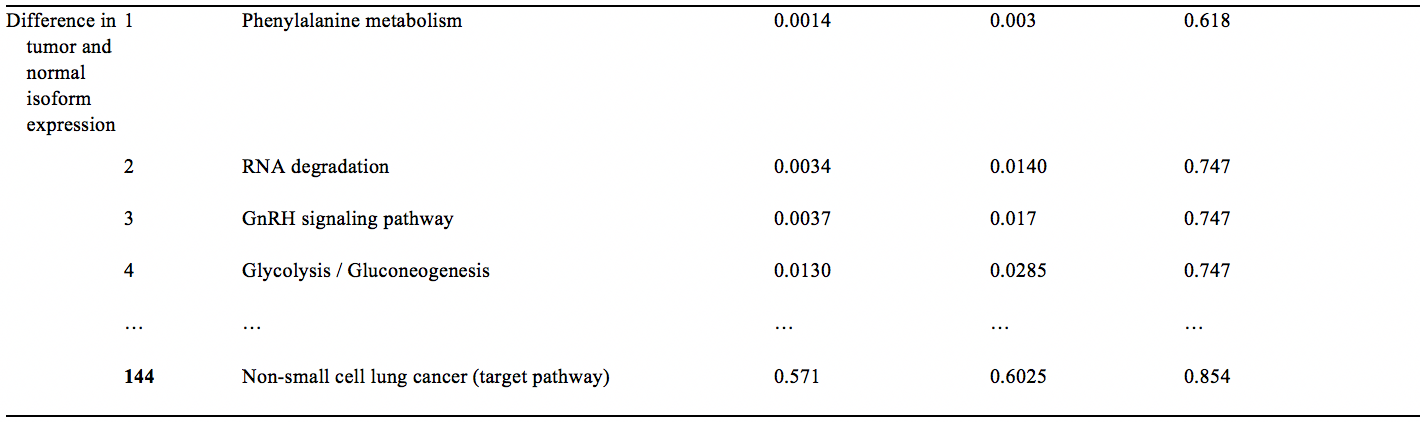
\includegraphics[keepaspectratio,width=\textwidth,height=0.8\textheight]{figures/table52.png}
\end{figure}
\end{frame}

\begin{frame}\frametitle{Study of subtype clustering inputs using Hellinger distances}
\begin{figure}[htb]
  \centering 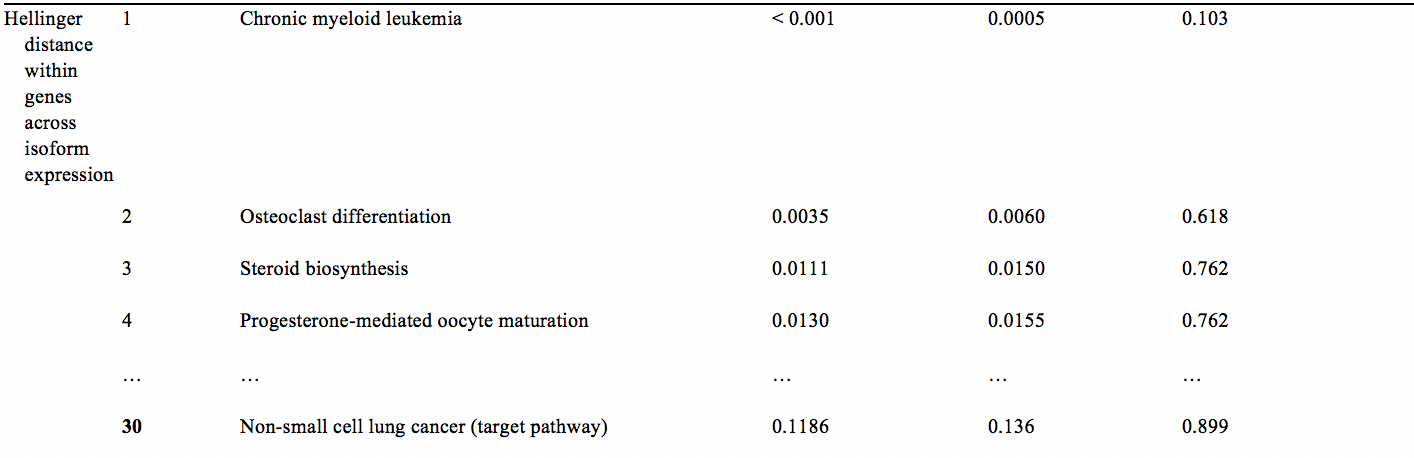
\includegraphics[keepaspectratio,width=\textwidth,height=0.8\textheight]{figures/table53.png}
\end{figure}
\end{frame}

\section{Concluding remarks}
%%\frame{\tableofcontents[currentsection]}

\begin{frame}\frametitle{Summary of contributions}
  \begin{enumerate}
  \item We developed the N-of-1-pathways Alternatively Spliced (N1PAS) framework.
    \item This will provide a single-subject method to detect alternatively spliced genetic pathways to enable precision medicine.
    \item We conducted Monte Carlo evaluations and find adequate false discovery rate control and impressive power to detect enriched pathways.
    \item We validated the method using target KEGG pathways.
    \item And applied N1PAS output to survival subtyping.
    \item Implemented an R package \url{https://github.com/grizant/n1pas/tree/master}.
  \end{enumerate}
\end{frame}

\begin{frame}\frametitle{Future directions}
  \begin{itemize}
  \item Extend the local false discovery method to better model the data at hand.
  \item Explore the theoretic properties of the model.
  \end{itemize}
\end{frame}


\begin{frame}\frametitle{Acknowledgments/gratitude:~collaborators \& funding}
  \vskip-10pt
\begin{columns}[T]
  \begin{column}{0.55\columnwidth}
    \begin{block}{U.~of Arizona}
      Yves A.~Lussier, MD\\
      Dillon Aberasturi, PhD candidate \\
      Colleen Kenost, ED
    \end{block}
%%     \begin{block}{WUST}
%%       Agnieszka Wylomanska, PhD, DSs \\
%%       Aleksandra Grzesiek, PhD candidate \\
%%       Everyone else involved
%%    \end{block}
    \begin{block}{UNR}
      Anna Panorska, PhD \\
      Tomasz Kozubowski, PhD
    \end{block}
    %%\begin{block}{Biologists}
    %%  Ikbel Achour, PhD\\
    %%  Joanne Berghout, PhD
    %%\end{block}
  \end{column}
  \begin{column}{0.45\columnwidth}
    \begin{block}{Grants/travel awards}
      UNR Office of Research \& Innovative\\
      The University of Arizona Health Sciences Center for Biomedical Informatics and Biostatistics\\
      NIH U01AI122275, HL132532, CA023074, 1UG3OD023171, 1S10RR029030
    \end{block}
  \end{column}
\end{columns}
\end{frame}


\begin{frame}\frametitle{Illustrative summary}
      \begin{figure}[htb]
  \centering
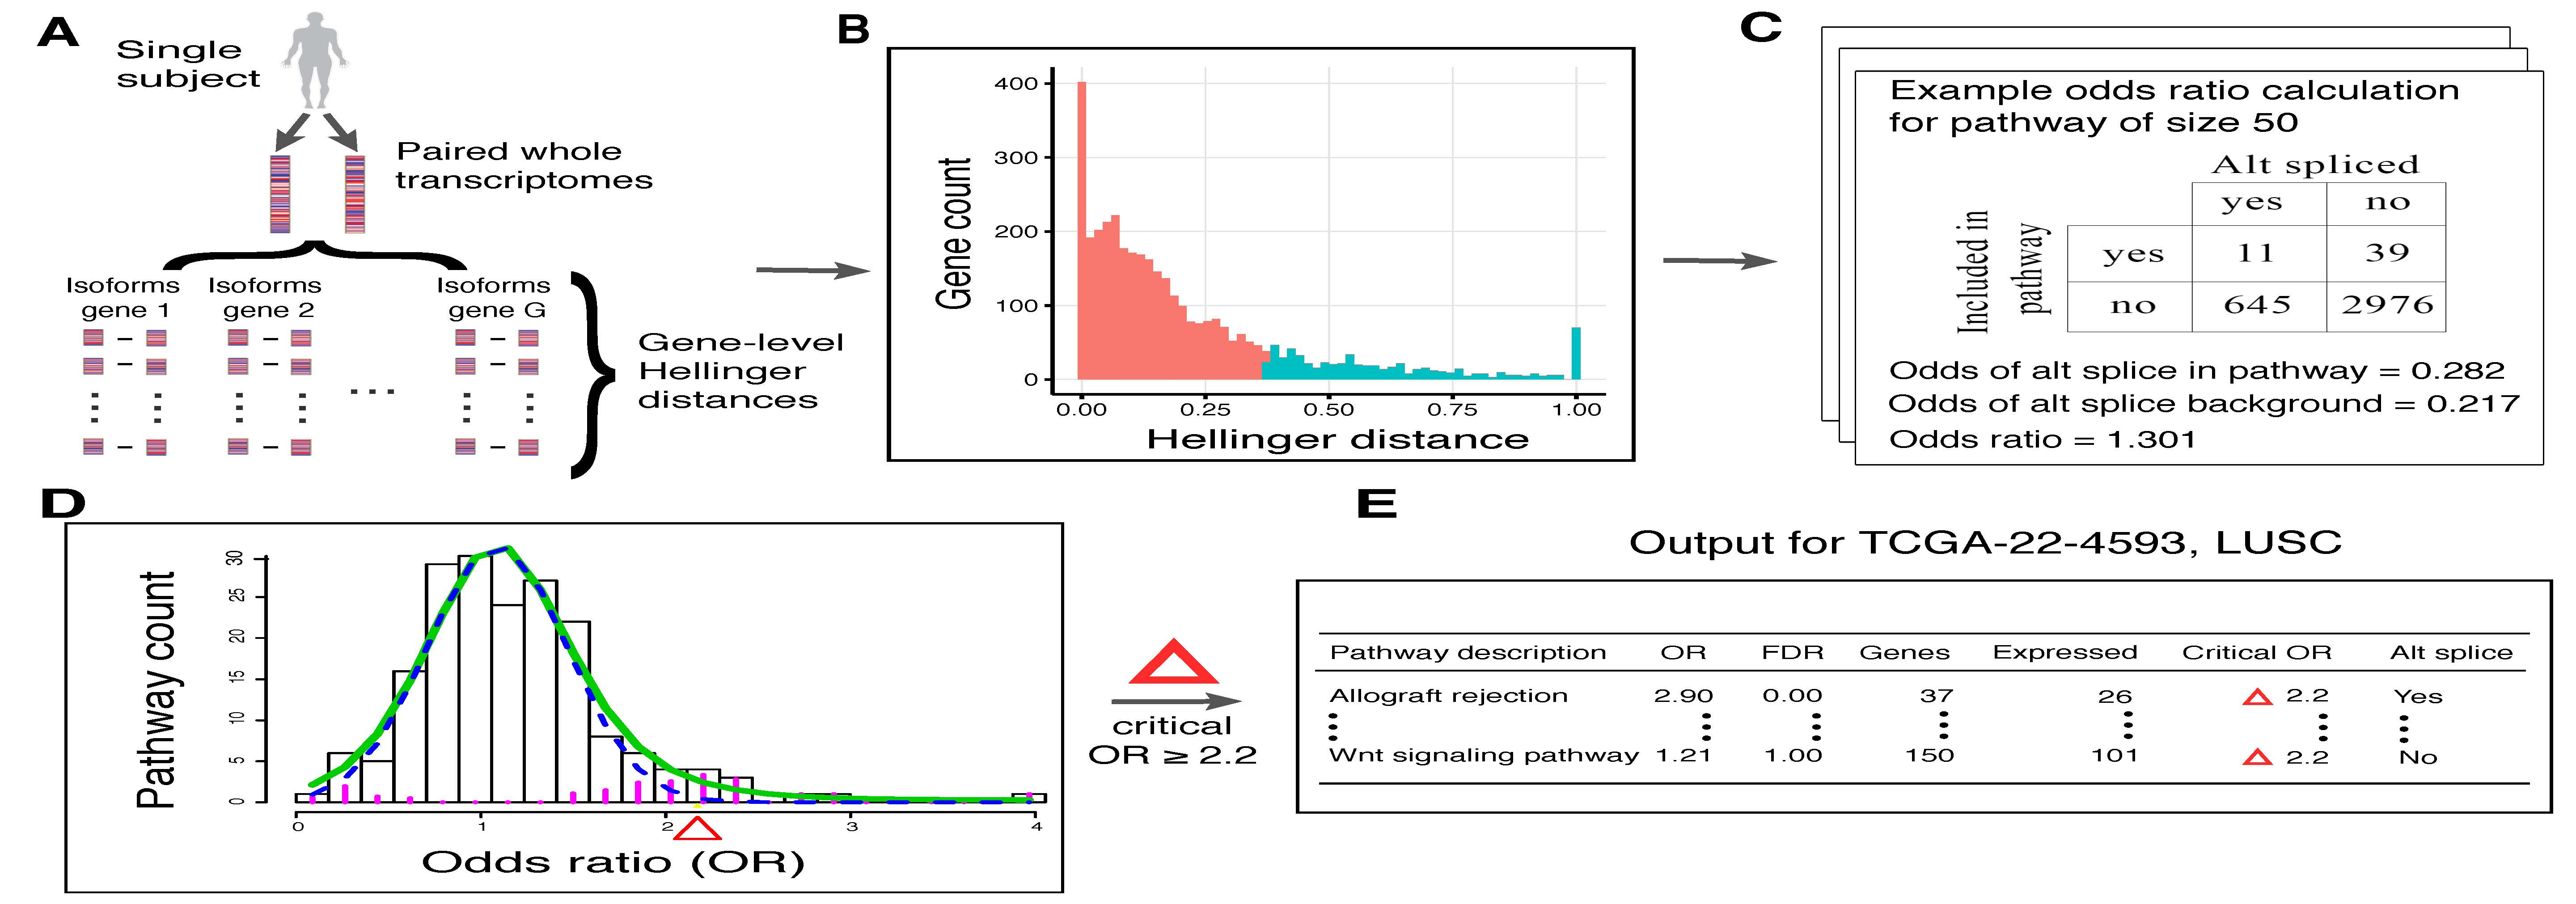
\includegraphics[keepaspectratio,width=\textwidth,height=.75\textheight]{figures/Figure1.jpg}
   \end{figure}
\end{frame}

%% Blank frame
\bgroup
\setbeamercolor{background canvas}{bg=black}
\begin{frame}[plain]{}
\end{frame}
\egroup

\appendix
\frame[allowframebreaks]{
  \printbibliography
}

\end{document}